%----------------------------------------------------------------------------------------
%	AAAI paper
%----------------------------------------------------------------------------------------


\chapter{Better bounds on the Adaptivity Gap of Influence Maximization under Full-Adoption feedback}\label{chap:background}
\fancyhead[L]{\textit{Chapter 3. Better Bounds on Adaptivity Gap}}


In this chapter, we consider the independent cascade model with full-adoption feedback, and show the first sub-linear upper bound on the adaptivity gap, (ratio between the optimal adaptive policy and the optimal non-adaptive policy [\ref{ag}]) that holds for general graphs. In detail, we show that the adaptivity gap is at most $\lceil n^{1/3}\rceil$ (Theorem~\ref{thrm2}), where $n$ is the number of nodes in the graph. Moreover, we tighten the upper bound on the adaptivity gap for in-arborescences by showing that it is at most $\frac{2e^2}{e^2-1}<\frac{2e}{e-1}$ (Theorem \ref{thrm1}).


Using similar techniques, we study the adaptivity gap of two classes of influence graphs: \emph{$\alpha$-bounded-degree graphs}, which is the class of influence graphs where the sum of node degrees higher than two is at most $\alpha$, and \emph{$(\beta,\gamma)$-bounded-activation graphs}, where the nodes are partitioned into influential nodes, which are at most $\beta$ nodes, and non-influential, where each of these nodes can infect at most $\gamma$ neighbours in expectation, where the value of $\gamma$ is less than 1. $\alpha$-bounded-degree graphs can be encountered in several graph topologies (see, for instance, Example \ref{exam1}), and $(\beta,\gamma)$-bounded-activation graphs are well-motivated by social networks in which most nodes have a limited power of influence. We show that the adaptivity gap of $\alpha$-bounded-degree and $(\beta,\gamma)$-bounded-activation graphs is upper-bounded by $\sqrt{\alpha}+O(1)$ and $\sqrt{\beta}+\frac{1}{1-\gamma}$ (Theorems \ref{thmlast} and \ref{thmlast2}) respectively, and these values are smaller than that of $O(n^{1/3})$ for several influence graph classes. Furthermore, in 0-bounded-degree graphs, i.e. undirected graphs in which each connected component is a path or a cycle, the adaptivity gap is at most $\frac{3e^3}{e^3-1}$ (Theorem~\ref{thm_0bou}). 
%

To prove our bounds, we introduce new techniques to connect adaptive policies with non-adaptive ones that might be of their own interest (further details are given in the paragraph ``General outline of the proof technique'' in Section \ref{sec_inarb}). In particular, we resort to a simple randomized {\em hybrid non-adaptive policy}, that differs from the main approaches previously used in adaptive influence maximization and other adaptive optimization problems:  (i) the {\em Poisson process} \cite{norris} combined with the {\em multi-linear extension of submodular set-functions} \cite{Calinescu11}, which represent the main probabilistic technique adopted by \citet{Asadpour16} and \citet{Chen2019}, and (ii) the {\em random walk on the decision tree} \cite{AdamczykGM15,sahil}, that is a tool applied by \citet{Gupta2017,Bradac19} and \citet{Peng2019}.

In the experimental section \ref{exp}, we take into account a cutting age non-adaptive greedy algorithm, called $TIM^+$, and design its adaptive version to compare their performance ratio, called the greedy adaptivity gap. To compute the efficiency of the seed set selected by $TIM^+$, we design another adaptive algorithm, which take as input the predetermined seed set selected by $TIM^+$, and running the adaptive algorithm on top of it. We observe that the ratio is closer to one, thus implying the efficiency of $TIM^+$ when compared to its adaptive counterpart.  

\subsection*{Related Works.}
Adaptivity gaps for the problem of maximizing stochastic monotone submodular functions have been studied by \citet{Asadpour16}. There exists a series of work engaged with adaptivity gaps for a two-step adaptive influence maximization problem~\cite{Badanidiyuru2016,Rubinstein2015, Seeman2013, Singer2016}. Gupta et al.~\cite{sahil, Gupta2017} and \citet{Bradac19} worked on the adaptivity gaps for stochastic probing. 

A recent line of studies~\cite{Chen2019, Chen2019a, Peng2019} focuses on finding the adaptivity gap on different graph classes using the classical feedback models. \citet{Peng2019} confirmed a conjecture of \citet{Golovin2011a}, which states that the adaptivity gap of the independent cascade model with myopic feedback is constant. In particular, they showed that the adaptivity gap belongs to $[\frac{e}{e-1}, 4]$. \citet{Chen2019a} introduced the greedy adaptivity gap, which compares the performance of the adaptive and the non-adaptive greedy algorithms. They show that the infimum of the greedy adaptivity gap is $1-\frac{1}{e}$ for every combination of diffusion and feedback models.

The most relevant related work to our results in this chapter is that of \citet{Chen2019}, as they derive upper and lower bounds on the adaptivity gap under the independent cascade model with full-adoption feedback, when the considered graphs are in-arborescences, out-arborescences, or one-directional bipartite graphs. In particular, they show that the adaptivity gaps of in-arborescences and out-arborescences are in the intervals $\left[ \frac{e}{e-1}, \frac{2e}{e-1}\right]$ and $\left[ \frac{e}{e-1}, 2\right]$ respectively, and they provide a tight bound of $\frac{e}{e-1}$ on the adaptivity gap of one-directional bipartite graphs. Under the more general triggering model, a constant upper bound of $2$ on the adaptivity gap of one-directional bipartite graphs was provided by \citet{Fujii2019}.


\subsection*{Contributions.}
Our main notable result in this chapter is the first sub-linear upper bound that holds for any graph. Specifically, we show that the adaptivity gap is upper-bounded by $\lceil n^{1/3}\rceil$, where $n$ is the number of nodes in the graph. Moreover, we improve over the known upper bound for in-arborescences from $2e/(e-1)\approx 3.16$ to $2e^2/(e^2-1)\approx 2.31$. 

Then, we study $\alpha$-bounded-degree graphs, that is the class of undirected graphs in which the sum of node degrees higher than two is at most $\alpha$, and show that the adaptivity gap is upper-bounded by $\sqrt{\alpha}+O(1)$; we also show that in 0-bounded-degree graphs, i.e. undirected graphs in which each connected component is a path or a cycle, the adaptivity gap is at most $3e^3/(e^3-1)\approx 3.16$. 

We also consider $(\beta,\gamma)$-bounded-activation graphs \cite{AIJ}, where all nodes but $\beta$ influence in expectation has at most $\gamma\in [0,1)$ neighbors each; for this class of influence graphs we show that the adaptivity gap is at most $\sqrt{\beta}+\frac{1}{1-\gamma}$. To prove our bounds, we introduce new techniques to relate adaptive policies with non-adaptive ones that might be of their own interest. 


Finally, we have some experiments to determine the performance efficiency of a specific widely used non-adaptive greedy algorithm, $TIM^+$. We build a greedy adaptive equivalent of $TIM^+$ and discuss about the quality of seed set generated by both the versions of $TIM^+$, the memory, and time overhead. We conclude that $TIM^+$ as a greedy non-adaptive algorithm performs quite well when compared to its adaptive counterpart and the main focus should be on the requirements of the computational costs to run these algorithms.

\subsection*{Organization of the Chapter.}
The preliminaries for this chapter is defined in Section~\ref{sec_prel}. Sections~\ref{sec_inarb}--\ref{sec_other} are devoted to the main technical contribution of the chapter, i.e., upper bounds on the adaptivity gap of in-arborescences, general graphs and other influence graphs ($\alpha$-bounded-degree and $(\beta,\gamma)$-bounded-activation graphs). Section \ref{exp} has some experiments comparing the results of $TIM^+$, adaptive greedy under $TIM^+$, and adaptive greedy with the seeds generated by $TIM^+$ for different network types and parameters under the IC and LT models. 

\section{Preliminaries}\label{sec_prel}
For two integers $h$ and $k$, $h\leq k$, let $[k]_h:=\{h,h+1,\ldots, k\}$ and $[k]:=[k]_1$. 

\paragraph*{Non-adaptive Influence Maximization} The {\em non-adaptive influence maximization problem under the IC model} is a computational problem that is defined as follows: given an influence graph $G$ and an integer $k\geq 1$, we are asked to find a set of seed nodes $S\subseteq V$ with $|S|=k$ such that $\sigma(S)$ is maximized. Without loss of generality, we assume that $k\in [n]$ and, since the objective function is monotone, $|S|=k$ for any solution $S$. A detailed overview is presented in Sections \ref{main}--\ref{nonada_sec} of Chapter \ref{chap:lit}. 

\paragraph*{Adaptive Influence Maximization} Differently from the non-adaptive setting, in which all the seed nodes are activated at the beginning and then the influence spread is observed, an {\em adaptive policy} activates the seeds sequentially in $k$ steps,
one seed node at each step, and the decision on the next seed node to select is based on the feedback resulting from the observed spread of the previously selected nodes. The feedback model considered in this work is {\em full-adoption}: when a node is selected, the adaptive policy observes its entire influence spread. 

An adaptive policy under the full-adoption feedback model is formally defined as follows. Given a live-edge graph $L$, the {\em realization} $\phi_L:V\rightarrow 2^V$ associated to $L$ assigns to each node $v\in V$ the value $\phi_L(v):=R(\{v\},L)$, i.e., the set of nodes activated by $v$ under a live-edge graph $L$. Given a set $S\subseteq V$, a {\em partial realization} $\psi:S\rightarrow 2^V$ is the restriction to $S$ for some realization, i.e., there exists a live-edge graph $L$ such that $\psi(v)=\phi_L(v)$ for any $v\in S$. Given a partial realization $\psi:S\rightarrow 2^V$, let $dom(\psi):=S$, i.e., $dom(\psi)$ is the domain of  partial realization $\psi$, let $R(\psi):=\bigcup_{v\in S}\psi(v)$, i.e., $R(\psi)$ is the set of nodes reached/activated by the diffusion process when the set of seed nodes is $S$, and let $f(\psi):=|R(\psi)|$. A partial realization $\psi'$ is a {\em sub-realization} of $\psi$ (or, equivalently,  $\psi'\subseteq \psi$), if $dom(\psi')\subseteq dom(\psi)$ and $\psi'(v)=\psi(v)$ for any $v\in dom(\psi')$. We observe that a partial realization $\psi$ can be equivalently represented as $\{(v,R(\{v\},L)):v\in dom(\psi)\}$ for some live-edge graph $L$. 

An adaptive policy $\pi$ takes as input a partial realization $\psi$ and, either returns a node $\pi(\psi)\in V$ and activates it as seed, or interrupts the activation of new seed nodes, e.g., by returning a string $\pi(\psi):=STOP$; furthermore, we assume (w.l.o.g.) that an adaptive policy $\pi$ chooses each seed based only on the observation of $R(\psi)$ (i.e., the set of nodes activated by the previous seeds) and $|dom(\psi)|$ (i.e., the number of seeds previously selected), that is, $\pi(\psi)=\pi(R(\psi),|dom(\psi)|)$. An adaptive policy $\pi$ can be run as in Algorithm \ref{ad_alg}. The {\em expected influence spread} of an adaptive policy $\pi$ is defined as $\sigma(\pi):=\mathbb{E}_L[f(\psi_{\pi,L})]$, i.e., it is the expected value (taken on all the possible live-edge graphs) of the number of nodes reached by the diffusion process at the end of Algorithm \ref{ad_alg}. We say that $|\pi|=k$ if policy $\pi$ always return a partial realization $\psi_{\pi,L}$ with $|dom(\psi_{\pi,L})|=k$. The {\em adaptive influence maximization problem under the IC model} is the computational problem that, given an influence graph $G$ and an integer $k\geq 1$, asks to find an adaptive policy $\pi$ that maximizes the expected influence spread $\sigma(\pi)$ subject to a constraint $|\pi|=k$. 
\begin{algorithm}[ht]
	\caption{Adaptive algorithm}
	\label{ad_alg}
	\begin{algorithmic}[1]
		\REQUIRE an influence graph $G$ and an adaptive policy $\pi$;
		\ENSURE a partial realization;
		\STATE let $L$ be the live-edge graph;
		\STATE let $\psi:=\emptyset$ (i.e., $\psi$ is the empty partial realization);
		\WHILE{$\pi(\psi)\neq STOP$}
		\STATE $v:=\pi(\psi)$;
		\STATE $\psi:=\psi\cup \{(v,R(\{v\},L))\}$;
		\ENDWHILE
		\RETURN $\psi_{\pi,L}:=\psi$;
	\end{algorithmic}
\end{algorithm}

\subsection*{Adaptivity Gap.} \label{ag}

Given an influence graph $G$ and an integer $k\geq 1$, let $OPT_N(G,k)$ (resp. $OPT_A(G,k)$) denote the optimal value of the non-adaptive (resp. adaptive) influence maximization problem with input $G$ and $k$. Given a class of influence graphs $\mathcal{G}$ and an integer $k\geq 1$, the {\em $k$-adaptivity gap} of $\mathcal G$ is defined as $$AG(\mathcal{G},k):=\sup_{G\in\mathcal{G}}\frac{OPT_A(G,k)}{OPT_N(G,k)},$$ and measures by how much does an adaptive policy outperform a non-adaptive solution for the influence maximization problem applied to influence graphs in $\mathcal{G}$, when the maximum number of seed nodes is $k$. The {\em adaptivity gap} of $\mathcal{G}$ is defined as $AG(\mathcal{G}):=\sup_{k\geq 1}AG(\mathcal{G},k)$. We observe that for $k=1$ or $n\leq k$ the $k$-adaptivity gap is trivially equal to 1, thus we omit such cases in the following. 

\section{Adaptivity Gap for In-arborescences}
\label{sec_inarb}
An {\em in-arborescence} is a graph $G=(V,E)$ that can be constructed from a rooted tree $T=(V,F)$, by adding an edge $(v,u)$ in $E$, if $u$ is a father of $v$ in tree $T$. By exploiting the shrinking boundary property, refer to figure \ref{fig:boundary} and lemma \ref{lemm2}, an upper bound of $\frac{2e}{e-1}\approx 3.16$ on the adaptivity gap of in-arborescences has been provided in \cite{Chen2019}. In this section we provide an improved upper bound for such graphs. 

\begin{figure}[ht]
\centering
\begin{subfigure}{0.4\textwidth}
    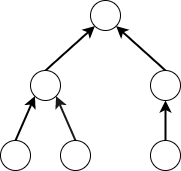
\includegraphics[width=0.8\linewidth]{GSSI_thesisProposal/figures/ina-2.png}
    \caption{An in-arborescence}
    \label{fig:ina}
\end{subfigure}
\hfill
\begin{subfigure}{0.4\textwidth}
    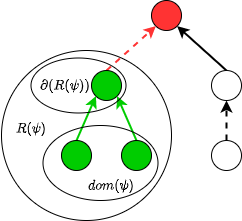
\includegraphics[width=0.8\linewidth]{GSSI_thesisProposal/figures/ina-1.png}
    \caption{Shrinking boundary of an in-arborescence}
    \label{fig:boundary}
\end{subfigure}
\caption{In-arborescence 
}
\label{fig:inar}
\end{figure}


\begin{theorem}\label{thrm1}
If $\mathcal{G}$ is the class of all the in-arborescences, then $$AG(\mathcal{G},k)\leq \frac{2}{1-(1-2/k)^k}\leq \frac{2e^2}{e^{2}-1}\approx 2.31,\ \forall k\geq 2.$$
\end{theorem}

Let $G=(V=[n],E,(p_{uv})_{(u,v)\in E})$ be an in-arborescence, where $n>k$ is the number of nodes. To show the claim of Theorem \ref{thrm1}, we need some preliminary notations and lemmas. Given a partial realization $\psi$, and a node $v\in V$, let 
$$\Delta(v|\psi):=\E_L[f(\psi\cup \{(v,R(\{v\},L))\})-f(\psi)|\psi\subseteq \phi_L],$$
i.e., $\Delta(v|\psi)$ is the expected increment of the influence spread due to node $v$ when the observed partial realization is $\psi$. We have the following claim (from \cite{Golovin2011a}), holding even for general graphs, whose proof is trivial. 

\begin{claim}[Adaptive Submodularity \cite{Golovin2011a}]\label{lem0}
Let $G$ be an arbitrary influence graph. For any partial realizations $\psi,\psi'$ of $G$ such that $\psi\subseteq \psi'$, and any node $v\notin R(\psi')$, we have that  $\Delta(v|\psi')\leq \Delta(v|\psi)$. 
\end{claim}


An adaptive policy $\pi$ is called {\em randomized} if, for any partial realization $\psi$, node $\pi(\psi)$ is not selected deterministically (in general), but randomly (according to a probability distribution $p_{\psi}$ depending on $\psi$). Given a vector $\bm y=(y_1,\ldots, y_n)$ such that $y_v\in [0,1]$ for any $v\in V$, we say that $\mathbb{P}(\pi)=\bm y$ if the probability that each node $v$ belongs to $dom(\psi_{\pi,L})$ is $y_v$, where $\psi_{\pi,L}$ is the partial realisation with policy $\pi$. Let $OPT_A(G,\bm y)$ be the optimal expected influence spread $\sigma(\pi)$ over all the randomized adaptive policies $\pi$ such that $\mathbb{P}(\pi)=\bm y$.\footnote{We observe that, if $\bm y$ is arbitrary, a deterministic policy $\pi$ verifying $\mathbb{P}(\pi)=\bm y$ might not exists, and the introduction of randomization solves this issue.}

Let $\pi^*$ be an optimal adaptive policy for the adaptive influence maximization problem (with $|\pi^*|=k$), and let $\bm x=(x_1,\ldots, x_n)$ be the vector such that $\mathbb{P}(\pi^*)=\bm x$. As $|\pi^*|=k$, we have that $\sum_{v\in V} x_v=k$. 

For any $t\in [k]_0$, let $S_t$ be the optimal set of $t$ seed nodes in the non-adaptive influence maximization problem, i.e., such that $OPT_N(G,t)=\mathbb{E}_L(|R(S_t,L)|)$. Let $\psi_{t,L}$ be the random variable denoting the sub-realisation of $\phi_L$ such that $dom(\psi_{t,L})=S_t$. Let $\rho$ be the random variable equal to node $v\in V$ with probability $x_v/k$. Observe that the above random variable is well-defined, as $\sum_{v\in V}(x_v/k)=k/k=1$. For any $t\in [k]$, let ${\psi}_{\rho,t,L}$ be the random variable denoting the sub-realisation of $\phi_L$ such that $dom({\psi}_{\rho,t,L})=S_{t-1}\cup\{\rho\}$.

\paragraph*{General outline of the proof technique} We observe that ${\psi}_{\rho,t,L}$ is the partial realization coming from the following  {\em hybrid non-adaptive policy}: initially, we activate the first $t-1$ seed nodes as in the optimal non-adaptive solution guaranteeing an expected influence spread of $OPT_N(G,t-1)$; then, we randomly choose a node $v$ according to random variable $\rho$ and we select $v$ as $t$-th seed node (if not already selected as seed). We use this hybrid non-adaptive policy as a main tool to obtain an improved upper bound on the adaptivity gap for in-arborescences. In Lemma \ref{lemm1}, holding even for general graphs, we relate the hybrid non-adaptive policy and the optimal non-adaptive solution, with the optimal adaptive policy. Lemma \ref{lemm1}, together with Lemma \ref{lemm2} (that is similar to Lemma 3.8 in~\cite{Chen2019}), is used in the main proof of the theorem to relate $OPT_N(G,t)$ with $OPT_A(G,k)$ for any $t\in [k]$, and this leads to our upper bound. 

The proof structure of Lemma \ref{lemm1} exhibits some similarities with Lemma 6 of \cite{Asadpour16} and Lemma 3.3 of \cite{Chen2019}, but in their approach, they relate non-adaptive policies based on the Poisson process and multi-linear extensions, with the optimal adaptive policy. One disadvantage of the Poisson process adopted in \cite{Chen2019} is that the number $X$ of seed nodes selected by the corresponding non-adaptive policy is equal to $k$ under expectation (i.e., $\mathbb{E}(X)=k$), and determining the expected influence spread w.r.t. random variable $X$ has implied a further loss in the final upper bound (see Lemma 3.9 and inequality (21) of Theorem 3.1 in \cite{Chen2019}). Instead, by using the hybrid-non-adaptive policy, we guarantee that the number of selected seed nodes at each step $t\in [k]$ is exactly equal to $t$,  independently from the considered random execution. This property allow us to avoid the expectations w.r.t. the number of selected seed nodes, and this leads to a further improvement of the resulting upper bound on the adaptivity gap.
\begin{lemma}\label{lemm1}
Let $G$ be an arbitrary influence graph. For any $t\in [k]$, and any fixed partial realization $\psi$ of $G$ such that $\mathbb{P}[\psi_{t-1,L}=\psi]>0$, we have $$OPT_A(G,k)\leq 
\sigma(R(\psi))+k\cdot \E_{L,\rho}\left[f({\psi}_{\rho,t,L})-f(\psi_{t-1,L})|\psi_{t-1,L}=\psi\right].$$
\end{lemma}
\begin{proof}
We have 
\begin{align}
&k\cdot \E_{L,\rho}\left[f({\psi}_{\rho,t,L})-f(\psi_{t-1,L})|\psi_{t-1,L}=\psi \right]\nonumber\\
=&k\cdot \sum_{v\in V}\mathbb{P}[\rho=v]\cdot \Delta(v|\psi)\nonumber\\
=&k\cdot \sum_{v\in V\setminus R(\psi)}\frac{x_v}{k}\cdot \Delta(v|\psi)\label{eq0}\\
=&\sum_{v\in V\setminus R(\psi)}x_v\cdot \Delta(v|\psi),\label{eq1}
\end{align}
where \eqref{eq0} holds since $\Delta(v|\psi)=0$ for any $v\in R(\psi)$. 

Let $\bm x'=(x_1',\ldots x_n')$ be the vector such that $x_v'=1$ if $v\in R(\psi)$, and $x_v'=x_v$ otherwise. As $x_v'\geq x_v$ for any $v\in V$ we have  
\begin{equation}\label{eq2}
OPT_A(G,k)\leq OPT_A(G,\bm x)\leq OPT_A(G,\bm x').
\end{equation}

Let $\pi'$ be the optimal randomized adaptive policy such that $\mathbb{P}(\pi')=\bm x'$. Policy $\pi'$ selects each node in $R(\psi)$ with probability $1$, thus we can assume that such seed nodes are selected at the beginning and that the adaptive policy starts by observing the resulting partial realization. Furthermore, we can assume that, for any partial realization $\psi'$, $\pi'$ does not select any node $v\in R(\psi')$, otherwise there is no increase of the influence spread. Given $j\in [n]$, let $\Delta'(j)$ denote the expected increment of the influence spread when $\pi'$ selects the $j$-th seed node (in order of selection, and without considering in the count the initial seeds of $R(\psi)$); analogously, let $\Delta'(j|v)$ denote the expected increment of the influence spread when $\pi'$ selects the $j$-th seed node, conditioned by the fact that the $j$-th seed is node $v$.\footnote{If an execution of $\pi'$ requires less than $j$ steps, we assume that the increase of the influence spread at step $j$ (that contributes to the expected values $\Delta'(j)$ and $\Delta'(j|v)$) is null.} We get
\begin{align}
 &OPT_A(G,\bm x')\nonumber\\
  =&\sigma(R(\psi))+\sum_j \Delta'(j)\nonumber\\
  =&\sigma(R(\psi))+\sum_j \sum_{v\in V\setminus R(\psi)}\mathbb{P}[\text{the $j$-th seed node is $v$}]\cdot \Delta'(j|v)\nonumber\\
  =&\sigma(R(\psi))+\sum_{v\in V\setminus R(\psi)}\sum_j \mathbb{P}[\text{the $j$-th seed node is $v$}]\cdot \Delta'(j|v)\nonumber\\
    =&\sigma(R(\psi))+\sum_{v\in V\setminus R(\psi)}\sum_j \mathbb{P}[\text{the $j$-th seed node is $v$}]\cdot\nonumber\\
    \cdot & \E_{\pi'}[\Delta(v|\psi')|\text{$v=\pi'(\psi')$ for some $\psi'\supseteq \psi$ observed at step $j$}]\nonumber\\
        \leq &\sigma(R(\psi))+\sum_{v\in V\setminus R(\psi)}\sum_j \mathbb{P}[\text{the $j$-th seed node is $v$}]\cdot \Delta(v|\psi)\label{eq3.0}\\
                =&\sigma(R(\psi))+\sum_{v\in V\setminus R(\psi)}\mathbb{P}[\text{$v$ is selected as seed}]\cdot \Delta(v|\psi)\nonumber\\
=& \sigma(R(\psi))+\sum_{v\in V\setminus R(\psi)}x_v'\cdot \Delta(v|\psi)\nonumber\\
= & \sigma(R(\psi))+\sum_{v\in V\setminus R(\psi)}x_v\cdot \Delta(v|\psi),\label{eq3}
\end{align}
where \eqref{eq3.0} holds since $\Delta(v|\psi')\leq \Delta(v|\psi)$ for any partial realization $\psi'\supseteq \psi$ by adaptive submodularity (Claim \ref{lem0}). By putting together \eqref{eq1}, \eqref{eq2}, and \eqref{eq3}, we get
\begin{align*}
& \sigma(R(\psi))+k\cdot \E_{L,\rho}\left[f({\psi}_{\rho,t,L})-f(\psi_{t-1,L})|\psi_{t-1,L}=\psi \right]\\
=& \sigma(R(\psi))+\sum_{v\in V\setminus R(\psi)}x_v\cdot \Delta(v|\psi)\\
\geq & OPT_A(G,\bm x')\\
\geq & OPT_A(G,k),
\end{align*}
thus showing the claim. 
\end{proof}

\begin{lemma}\label{lemm2}
If the input influence graph $G$ is an in-arborescence, then $$
\sigma(R(\psi_{t-1,L}))\leq f(\psi_{t-1,L})+OPT_N(G,t-1)$$
  for any live-edge graph $L$ and $t\in [k]$. 
\end{lemma}
\begin{proof}
Given a subset $U\subseteq V$, let $\partial U:=\{u\in U:\exists (u,v)\in E,v\notin U\}$. We have that $\sigma(R(\psi))\leq |R(\psi)|+\sigma(\partial R(\psi))=f(\psi)+\sigma(\partial R(\psi))$ for any partial realization $\psi$. Thus, to show the claim, it suffices to show that $\sigma(\partial R(\psi_{t-1,L}))\leq OPT_N(G,t-1)$. For in-arborescences, we have that $|\partial R(\psi_{t-1,L})|\leq |dom(\psi_{t-1,L})|=t-1$, thus $\sigma(\partial R(\psi_{t-1,L}))\leq OPT_N(G,t-1)$.
\end{proof}
Armed with the above lemmas, we can now prove Theorem~\ref{thrm1}.

\begin{proof}[Proof of Theorem~\ref{thrm1}]
For any $t\in [k]$, we have
\begin{align}
&k\cdot (OPT_N(G,t)-OPT_N(G,t-1))\nonumber\\
=&k\cdot (\sigma(S_t)-\sigma(S_{t-1}))\nonumber\\
=&k\cdot (\E_L[f(\psi_{t,L})]-\E_L[f(\psi_{t-1,L})])\nonumber\\
\geq &k\cdot (\E_{L,\rho}[f({\psi}_{\rho,t,L})]-\E_L[f(\psi_{t-1,L})])\label{eqthm1.0}\\
= &k\cdot (\E_{L,\rho}[f({\psi}_{\rho,t,L})]-\E_{L,\rho}[f(\psi_{t-1,L})])\nonumber\\
=&k\cdot \E_{L,\rho}[f({\psi}_{\rho,t,L})-f(\psi_{t-1,L})]\nonumber\\
=& \E_{\psi_{t-1,L}}\left[k\cdot \E_{L,\rho}[f({\psi}_{\rho,t,L})-f(\psi_{t-1,L})|\psi_{t-1,L}]\right]\nonumber\\
\geq &\E_{\psi_{t-1,L}}[OPT_A(G,k)-\sigma(R(\psi_{t-1,L}))]\label{eqthm1}\\
\geq &\E_{\psi_{t-1,L}}[OPT_A(G,k)-f(\psi_{t-1,L})-OPT_N(G,t-1)]\label{eqthm3}\\
=& \E_{\psi_{t-1,L}}[OPT_A(G,k)]-\E_{\psi_{t-1,L}}[f(\psi_{t-1,L})]-\E_{\psi_{t-1,L}}[OPT_N(G,t-1)]\nonumber\\
= &OPT_A(G,k)-\sigma(S_{t-1})-OPT_N(G,t-1)\nonumber\\
= &OPT_A(G,k)-2\cdot OPT_N(G,t-1)\label{eqthm4},
\end{align}
where \eqref{eqthm1.0} holds since $dom(\psi_{t,L})$ is the optimal set of $t$ seed nodes for the non-adaptive influence maximization problem, \eqref{eqthm1} comes from Lemma \ref{lemm1}, and \eqref{eqthm3} comes from Lemma~\ref{lemm2}. Thus, by \eqref{eqthm4}, we get $k\cdot (OPT_N(G,t)-OPT_N(G,t-1))\geq OPT_A(G,k)-2\cdot OPT_N(G,t-1)$, that after some manipulations leads to the following recursive relation:
\begin{equation}
OPT_N(G,t)\geq \frac{1}{k}\cdot OPT_A(G,k)+\left(1-\frac{2}{k}\right)\cdot OPT_N(G,t-1),\ \forall t\in [k].\label{fundeqthm}
\end{equation}
%
By applying \eqref{fundeqthm} iteratively, we get
\begin{align*}
    OPT_N(G,k)&\geq \frac{1}{k}\cdot \sum_{t=0}^{k-1}\left(1-\frac{2}{k}\right)^{t}\cdot OPT_A(G,k)=\frac{1-\left(1-2/k\right)^k}{2}\cdot OPT_A(G,k),
\end{align*}
that leads to 
\begin{equation*}
\frac{OPT_A(G,k)}{OPT_N(G,k)}\leq \frac{2}{1-(1-2/k)^k}\leq \frac{2}{1-e^{-2}} = \frac{2e^2}{e^{2}-1},
\end{equation*}
and this shows the claim. 
\end{proof}
\section{Adaptivity Gap for General Influence  Graphs}\label{sec_gen}
In this section, we exhibit upper bounds on the $k$-adaptivity gap of general graphs. In the following theorem, we first give an upper bound that is linear in the number of seed nodes.
\begin{theorem}\label{lemk}
Given an arbitrary class of influence graphs $\mathcal{G}$ and $k\geq 2$, we get $AG(\mathcal{G},k)\leq k$. 
\end{theorem}
\begin{proof}
Let $G=(V=[n],E,(p_{uv})_{(u,v)\in E})$ be an arbitrary influence graph. Let $\pi^*$ be an optimal adaptive policy subject to $|\pi^*|=k$, and let $\psi_{t,\pi^*,L}$ be the partial realization observed when the $t$-th seed node has been selected by Algorithm \ref{ad_alg} with policy $\pi^*$. Fix $t\in [k]$, a partial realization $\psi$ such that $\mathbb{P}[\psi_{t,\pi^*,L}=\psi]>0$, and let $v=\pi^*(\psi)$ be the node selected by policy $\pi^*$ under partial realization $\psi$. We have that
\begin{align}
&\E_{L}[f(\psi_{t,\pi^*,L})-f(\psi_{t-1,\pi^*,L})|\psi_{t-1,\pi^*,L}=\psi]\nonumber\\
=&\Delta(v|\psi)\nonumber\\
\leq & \Delta(v|\emptyset)\label{eq1lemk}\\
=&\sigma(\{v)\})\nonumber\\
\leq & OPT_N(G,1),\label{eq2lemk}
\end{align}
where \eqref{eq1lemk} holds by adaptive submodularity (Claim  \ref{lem0}). Thus, we get
\begin{align}
OPT_A(G,k)=&\E_{L}[f(\psi_{k,\pi^*,L})]\nonumber\\
=&\sum_{t=1}^k \E_{L}[f(\psi_{t,\pi^*,L})-f(\psi_{t-1,\pi^*,L})]\nonumber\\
=&\sum_{t=1}^k \E_{\psi_{t-1,\pi^*,L}}[\E_L[f(\psi_{t,\pi^*,L})-f(\psi_{t-1,\pi^*,L})|\psi_{t-1,\pi^*,L}]]\nonumber\\
\leq &k\cdot\E_{\psi_{t-1,\pi^*,L}}[OPT_N(G,1)]\label{eq3lemk}\\
=&k\cdot OPT_N(G,1)\nonumber\\
\leq &k\cdot OPT_N(G,k),
\end{align}
where \eqref{eq3lemk} comes from \eqref{eq2lemk}, and the claim follows.
\end{proof}
In the next theorem we give an upper bound on the adaptivity gap that is sublinear in the number of nodes of the considered graph.

When considering general graphs having a bounded number of nodes, we get an upper bound on the adaptivity gap that is sublinear in the maximum number of nodes of the considered graphs. 

\begin{theorem}\label{thrm2}
If $\mathcal{G}$ is the class of influence graphs having at most $n$ nodes, we get $AG(\mathcal{G})\leq \lceil n^{1/3}\rceil .$ 
\end{theorem}

Let $G=(V,E,(p_{uv})_{(u,v)\in E})$ be the input influence graph. To show Theorem \ref{thrm2}, we recall the preliminary notations considered for the proof of Theorem \ref{thrm1}, and we give a further preliminary lemma. 
\begin{lemma}\label{lemthm2}
Given a set $U\subseteq V$ of cardinality $h\geq k$, we have $\sigma(U)\leq \frac{h}{k}\cdot OPT_N(G,k).$
\end{lemma}
\begin{proof}
For any $t\in [h]_0$, let $U_t:=\emptyset$ if $t=0$, and $U_t:=U_{t-1}\cup\{v_t\}$, where $v_t\in\arg\max_{v\in U\setminus U_{t-1}}(\sigma(U_{t-1}\cup\{v\})-\sigma(U_{t-1})).$ We have that $\Delta_t:=\sigma(U_{t})-\sigma(U_{t-1})$ is non-increasing in $t\in [h]$. Indeed, given $t\in [k-1]$, we have that
\begin{align}
\Delta_{t+1}=&\sigma(U_{t+1})-\sigma(U_{t})\nonumber\\
=&\sigma(U_{t}\cup\{v_{t+1}\})-\sigma(U_{t})\nonumber\\
\leq &\sigma(U_{t-1}\cup\{v_{t+1}\})-\sigma(U_{t-1})\label{eq1lem2thm2}\\
\leq &\max_{v\in U\setminus U_{t-1}}(\sigma(U_{t-1}\cup\{v\})-\sigma(U_{t-1}))\nonumber\\
=&\sigma(U_{t-1}\cup\{v_{t}\})-\sigma(U_{t-1})\nonumber\\
=&\Delta_t,\label{eq2lem2thm2}
\end{align}
where \eqref{eq1lem2thm2} holds since $\sigma$ is a submodular set-function (see \cite{Kempe2015}). Thus, we necessarily have 
\begin{align}
\frac{\sigma(U)}{h}=&\frac{\sum_{t=1}^h\Delta_t}{h}\nonumber\\
\leq &\frac{\sum_{t=1}^k\Delta_t\left(h/k\right)}{h}\label{eq3lem2thm2}\\
=&\frac{\sum_{t=1}^k\Delta_t}{k}\nonumber\\
=&\frac{\sigma(U_k)}{k}\nonumber\\
\leq &\frac{OPT_N(G,k)}{k},\label{eq4lem2thm2}
\end{align}
where \eqref{eq3lem2thm2} comes from \eqref{eq2lem2thm2}. By \eqref{eq4lem2thm2}, the claim follows.
\end{proof}
We use Theorem~\ref{lemk} and Lemma~\ref{lemthm2} to show Theorem~\ref{thrm2}.

\begin{proof}[Proof of Theorem~\ref{thrm2}]
We assume w.l.o.g. that $k>\lceil n^{1/3}\rceil $ and that $OPT_N(G,k)<(\lceil n^{1/3}\rceil)^2$. Indeed, if $k\leq  \lceil n^{1/3}\rceil $, by Theorem \ref{lemk} the claim holds, and if $OPT_N(G,k)\geq (\lceil n^{1/3}\rceil)^2$, then $\frac{OPT_A(G,k)}{OPT_N(G,k)}\leq \frac{|V|}{OPT_N(G,k)}\leq \frac{n}{(\lceil n^{1/3}\rceil)^2}\leq \lceil n^{1/3}\rceil $, and the claim holds as well. 
For any $t\in [k]$, we have
\begin{align}
&k\cdot (OPT_N(G,t)-OPT_N(G,t-1))\nonumber\\
\geq &k\cdot (\E_{L,\rho}[f({\psi}_{\rho,t,L})]-\E_{L,\rho}[f(\psi_{t-1,L})])\nonumber\\
=& \E_{\psi_{t-1,L}}\left[k\cdot \E_{L,\rho}[f({\psi}_{\rho,t,L})-f(\psi_{t-1,L})|\psi_{t-1,L}]\right]\nonumber\\
\geq &\E_{\psi_{t-1,L}}[OPT_A(G,k)-\sigma(R(\psi_{t-1,L}))]\label{eqthm12}\\
=&\E_{\psi_{t-1,L}}[OPT_A(G,k)]-\E_{\psi_{t-1,L}}[\sigma(R(\psi_{t-1,L}))]\nonumber\\
\geq &\E_{\psi_{t-1,L}}[OPT_A(G,k)]-\E_{\psi_{k,L}}[\sigma(R(\psi_{k,L}))]\nonumber\\
\geq &\E_{\psi_{t-1,L}}[OPT_A(G,k)]-\E_{\psi_{k,L}}\left[\frac{|R(\psi_{k,L})|}{k}\cdot OPT_N(G,k)\right]\label{eqthm32}\\
= &OPT_A(G,k)-\frac{\E_{\psi_{k,L}}[|R(\psi_{k,L})|]}{k}\cdot OPT_N(G,k)\nonumber\\
\geq  &OPT_A(G,k)-\frac{\E_{\psi_{k,L}}[|R(\psi_{k,L})|]}{\lceil n^{1/3}\rceil+1}\cdot ((\lceil n^{1/3}\rceil)^2-1)\label{eqthm42}\\
=&OPT_A(G,k)-(\lceil n^{1/3}\rceil-1)\cdot \E_{\psi_{k,L}}[|R(\psi_{k,L})|]\nonumber\\
=&OPT_A(G,k)-(\lceil n^{1/3}\rceil-1)\cdot OPT_N(G,k)\label{eqthm52},
\end{align}
where \eqref{eqthm12} comes from Lemma \ref{lemm1}, \eqref{eqthm32} comes from Lemma \ref{lemthm2}, and \eqref{eqthm42} comes from the hypothesis $k>\lceil n^{1/3}\rceil $ and $OPT_N(G,k)<(\lceil n^{1/3}\rceil)^2$. By \eqref{eqthm52}, we get $OPT_N(G,t)-OPT_N(G,t-1)
\geq (OPT_A(G,k)-(\lceil n^{1/3}\rceil-1)\cdot OPT_N(G,k))/k$ for any $t\in [k]$, and by summing such inequality over all $t\in [k]$, we get
\begin{align}
& OPT_N(G,k)\nonumber\\
=&\sum_{t=1}^k (OPT_N(G,t)-OPT_N(G,t-1))\nonumber\\
\geq &\sum_{t=1}^k\frac{OPT_A(G,k)-(\lceil n^{1/3}\rceil-1)\cdot OPT_N(G,k)}{k}\nonumber\\
=&OPT_A(G,k)-(\lceil n^{1/3}\rceil-1)\cdot OPT_N(G,k).\label{eqthm62}
\end{align}
Finally, \eqref{eqthm62} implies that $OPT_A(G,k)\leq \lceil n^{1/3}\rceil \cdot OPT_N(G,k)$, and this shows the claim. 
\end{proof}
\section{Adaptivity Gap for Other Influence Graphs}\label{sec_other}
In this section, we extend the results obtained in Theorem \ref{thrm1}, and we get upper bounds on the adaptivity gap of other classes of influence graphs. 
\subsection {$\alpha$-bounded-degree graphs} \label{sec_alpha}
We first consider the class of {\em $\alpha$-bounded-degree graphs}: a class of undirected influence graphs parametrized by an integer $\alpha\geq 0$ that includes several known graph topologies. In the following, when we refer to undirected influence graphs, we assume that, for any undirected edge $\{u,v\}$, there are two directed edges $(u,v)$ and $(v,u)$ having respectively two (possibly) distinct probabilities $p_{uv}$ and $p_{vu}$. 

Given an undirected graph $G=(V,E)$ and a node $v\in V$, let $deg_v(G)$ denote the degree of node $v$ in graph $G$. Given an integer $\alpha\geq 0$, an influence graph $G=(V,E,(p_{uv})_{(u,v)\in E})$ is an {\em $\alpha$-bounded-degree graph} if it is undirected and $\sum_{v\in V:deg_v(G)>2}deg_v(G)\leq \alpha,$ i.e., the sum all the node degrees higher than $2$ is at most $\alpha$; we observe that the definition of $\alpha$-bounded degree graphs does not depends on the influence probabilities, but on the graph topology only. 
\begin{example}\label{exam1}
Given an undirected graph $G$, a simple subpath $P$ (resp. cycle $C$) of $G$ is {\em standard} if all the nodes of $P$ but the first and the last one (resp. all the nodes of $C$) have degree $2$. The {\em standard contraction} of $G$ is the multigraph $G'$ obtained by replacing each maximal simple subpath $P=(v_1,\ldots, v_t)$ of $G$ such that $deg_{v_2}(G)=deg_{v_3}(G)=deg_{v_{t-1}}(G)=2$, with an edge and by deleting each simple cycle $C=(v_1,v_2,\ldots, v_{t-1},v_t=v_1)$ such that $deg_{v_2}(G)=deg_{v_3}(G)=deg_{v_{t-1}}(G)=2$. There are several interesting classes of $\alpha$-bounded-degree graphs characterized by the topological structure of their standard contraction:
\begin{itemize}
\item The set of $0$-bounded-degree graphs is made of all the graphs $G$ such that each connected component of $G$ is either an undirected path or an undirected cycle; equivalently, the set of $0$-bounded-degree graphs is made of all the graphs $G$ whose standard contraction is the (possibly empty) union of several disconnected edges.
\item If the standard contraction of a graph $G$ is homeomorphic to a star with $h$ edges, then $G$ is a $h$-bounded-degree graph.
\item If the standard contraction of a graph $G$ is homeomorphic to a parallel-link multigraph with $h$ edges, then $G$ is a $2h$-bounded-degree graph.
\item If the standard contraction of a graph $G$ is homeomorphic to a cycle with $h$ chords, then $G$ is a $6h$-bounded-degree graph.
\item If the standard contraction of a graph $G$ is homeomorphic to a clique with $h$ nodes, then $G$ is a $h(h-1)$-bounded-degree graph.
\end{itemize}
\end{example}
In the following, we provide an upper bound on the adaptivity gap of $\alpha$-bounded-degree graphs for any $\alpha\geq 0$. 
\begin{theorem}\label{thmlast}
Given $\alpha\geq 0$, let $\mathcal{G}$ be the class of  $\alpha$-bounded-degree graphs. Then 
$$AG(\mathcal{G},k)\leq \min\left\{k,\frac{\alpha}{k}+2+ \frac{1}{1-(1-1/k)^k}\right\}\leq \frac{\sqrt{4(e-1)^2\alpha+(3e-2)^2}+3e-2}{2(e-1)}$$
for any $k\geq 2$, i.e., $AG(\mathcal{G})\leq \sqrt{\alpha}+O(1)$. 
\end{theorem}

Let $G=(V=[n],E,(p_{uv})_{(u,v)\in E})$ be an $\alpha$-bounded-degree graph, and we recall the preliminary notations from Theorem \ref{thrm1}. The proof of Theorem \ref{thmlast} is a non-trivial generalization of Theorem \ref{thrm1}. In particular, the proof resorts to Theorem \ref{lemk} to get the upper bound of $k$, and, by following the approach of Theorem \ref{thrm1}, the following technical lemma is used in place of Lemma \ref{lemm2} to get the final upper bound. 
\begin{lemma}\label{lemlast}
When the input influence graph $G$ is an $\alpha$-bounded-degree graph with $\alpha\geq 0$, we have that $
\sigma(R(\psi_{t-1,L}))\leq f(\psi_{t-1,L})+\left(\frac{\alpha}{k}+2\right)\cdot OPT_N(G,k)$ for any $t\in [k]$ and live-edge graph $L$.
\end{lemma}
\begin{proof}%[Proof of Lemma \ref{lemlast}]
Given a subset $U\subseteq V$, let $\partial U:=\{u\in U: \exists (u,v)\in E,v\notin U\}$. We have that $\sigma(R(\psi))\leq |R(\psi)|+\sigma(\partial R(\psi))=f(\psi)+\sigma(\partial R(\psi))$ for any partial realization $\psi$. Thus, to show the claim, it suffices to show that 
\begin{equation*}%\label{eqlast1}
\sigma(\partial R(\psi_{t-1,L}))\leq \left(\frac{\alpha}{k}+2\right)\cdot OPT_N(G,k).
\end{equation*}
Let $U\subseteq V$ such that $U$ has at most $k$ connected components. Let $A$ be the set of connected components containing at least one node of degree higher than $2$, and let $B$ be the set of the remaining components, i.e., containing nodes with degree in $[2]_0$ only. By definition of $A$ and $B$, we necessarily have that $|\partial A|\leq \sum_{v\in V:deg_v(G)>2}deg_v(G)\leq \alpha$ and $|\partial B|\leq 2k$. Thus $|\partial U|\leq |\partial A|+|\partial B|\leq \alpha+2k$, and the next claim follows.
\begin{claim}\label{lastclaim}
Given a subset $U\subseteq V$ made of at most $k$ connected components, then $|\partial U|\leq \alpha+2k$. 
\end{claim}
Now, we have that
\begin{align}
\sigma(\partial R(\psi_{t-1,L}))\leq & \sigma(\partial R(\psi_{k,L}))\nonumber\\
\leq & \frac{|\partial R(\psi_{k,L})|}{k}\cdot OPT_N(G,k)\label{lastlem_eq2}\\
\leq & \frac{\alpha+2k}{k}\cdot OPT_N(G,k),\label{lastlem_eq3}
\end{align}
where \eqref{lastlem_eq2} comes from Lemma \ref{lemthm2}, and \eqref{lastlem_eq3} holds since $R(\psi_{k,L})$ contains at most $k$ connected components and because of Claim \ref{lastclaim}. Thus, by \eqref{lastlem_eq3}, the claim of the lemma follows. 
\end{proof}

We can now prove Theorem~\ref{thmlast}.
\begin{proof}[Proof of Theorem~\ref{thmlast}]
For any $t\in [k]$, we have
\begin{align}
&k\cdot (OPT_N(G,t)-OPT_N(G,t-1))\nonumber\\
\geq &k\cdot (\E_{L,\rho}[f({\psi}_{\rho,t,L})]-\E_{L,\rho}[f(\psi_{t-1,L})])\nonumber\\
=& \E_{\psi_{t-1,L}}\left[k\cdot \E_{L,\rho}[f({\psi}_{\rho,t,L})-f(\psi_{t-1,L})|\psi_{t-1,L}]\right]\nonumber\\
\geq &\E_{\psi_{t-1,L}}[OPT_A(G,k)-\sigma(R(\psi_{t-1,L}))]\label{eqthm1_last}\\
\geq &\E_{\psi_{t-1,L}}\left[OPT_A(G,k)-f(\psi_{t-1,L})-\left(\frac{\alpha}{k}+2\right)OPT_N(G,k)\right]\label{eqthm3_last}\\
=& \E_{\psi_{t-1,L}}[OPT_A(G,k)]-\E_{\psi_{t-1,L}}[f(\psi_{t-1,L})]-\left(\frac{\alpha}{k}+2\right)\cdot\E_{\psi_{t-1,L}}\left[OPT_N(G,k)\right]\nonumber\\
= &OPT_A(G,k)-\sigma(S_{t-1})-\left(\frac{\alpha}{k}+2\right)\cdot OPT_N(G,k)\nonumber\\
= &OPT_A(G,k)-\left(\frac{\alpha}{k}+2\right)\cdot OPT_N(G,k)-OPT_N(G,t-1)\label{eqthm4_last},
\end{align}
where \eqref{eqthm1_last} comes from Lemma \ref{lemm1} and \eqref{eqthm3_last} comes from Lemma \ref{lemlast}. Thus, by \eqref{eqthm4_last}, we get the following recursive relation:
\begin{equation}\label{fundeqthm_last}
OPT_N(G,t)\geq \frac{1}{k}\left(OPT_A(G,k)-\left(\frac{\alpha}{k}+2\right)OPT_N(G,k)\right)+\left(1-\frac{1}{k}\right)OPT_N(G,t-1),
\end{equation}
for any $t\in [k]$. By applying iteratively \eqref{fundeqthm_last}, we get 
\begin{align*}
OPT_N(G,k)
&\geq \frac{1}{k}\cdot \left(OPT_A(G,k)-\left(\frac{\alpha}{k}+2\right)\cdot OPT_N(G,k)\right)\cdot \sum_{t=0}^{k-1} \left(1-\frac{1}{k}\right)^j\\
&=\left(OPT_A(G,k)-\left(\frac{\alpha}{k}+2\right)\cdot OPT_N(G,k)\right)\cdot \left(1-\left(1-\frac{1}{k}\right)^k\right),
\end{align*}
that, after some manipulations, leads to 
\begin{equation}\label{semifinal_bound}
%\frac{OPT_A(G,k)}{OPT_N(G,k)}\leq \frac{(\alpha/k+2)(1-(1-1/k)^k)+1}{1-(1-1/k)^k}.
\frac{OPT_A(G,k)}{OPT_N(G,k)}\leq \frac{\alpha}{k}+2+ \frac{1}{1-(1-1/k)^k} \leq \frac{\alpha}{k}+2+ \frac{1}{1-e^{-1}}~.
\end{equation}
By Theorem \ref{lemk}, we have that $\frac{OPT_A(G,k)}{OPT_N(G,k)}\leq k$, thus, by \eqref{semifinal_bound}, we get 
\begin{align}
\frac{OPT_A(G,k)}{OPT_N(G,k)}\leq & \min\left\{k, \frac{\alpha}{k}+2+ \frac{1}{1-(1-1/k)^k} \  \right\}\nonumber\\
\leq & \min\left\{k, \frac{\alpha}{k}+2+ \frac{1}{1-e^{-1}} \  \right\}\nonumber\\
\leq  & \frac{\sqrt{4(e-1)^2\alpha+(3e-2)^2}+3e-2}{2(e-1)}\label{last_eqq},
\end{align}
where \eqref{last_eqq} is equal to the real value of $k\geq 0$ such that $k=\frac{\alpha}{k}+2+ \frac{1}{1-e^{-1}}$. By \eqref{last_eqq} the claim follows. 
\end{proof}

For the particular case of $0$-bounded-degree graphs, the following theorem provides a better  upper bound on the adaptivity gap.
\begin{theorem}\label{thm_0bou}
Let $\mathcal{G}$ be the class of $0$-bounded-degree graphs. Then $$AG(\mathcal{G},k)\leq\min\left\{k,\frac{3}{1-(\max\{0,1-3/k\})^k}\right\}\leq \frac{3e^3}{e^{3}-1}\approx 3.16,$$ 
for any $k\geq 2$. 
\end{theorem}
The proof of Theorem \ref{thm_0bou} is similar to that of Theorem \ref{thrm1}. Let $G=(V=[n],E,(p_{uv})_{(u,v)\in E})$ be a $0$-bounded-degree graph. We recall the notation from Theorem \ref{thrm1} and we give the following preliminary lemma, whose proof is analogue to that of Lemma \ref{lem2}. 
\begin{lemma}\label{lem_0bou}
When the input influence graph $G$ is a $0$-bounded-degree graph, we have  
\begin{equation}
\sigma(R(\psi_{t-1,L}))\leq f(\psi_{t-1,L})+2\cdot OPT_N(G,t-1),
\end{equation}
for any $t\in [k]$ and live-edge graph $L$.
\end{lemma}
\begin{proof}
As in Lemma \ref{lemm2}, we show that $\sigma(\partial R(\psi_{t-1,L}))\leq 2\cdot OPT_N(G,t-1)$. First of all, we assume that $t\geq 2$, otherwise $\sigma(R(\psi_{t-1,L}))$ and the claim holds. By Lemma \ref{lemthm2}, we have that $\sigma(\partial R(\psi_{t-1,L}))\leq \frac{|\partial R(\psi_{t-1,L})|}{t-1}\cdot OPT_N(G,t-1)$. As $G$ is a $0$-bounded-degree graph, we have that $|\partial R(\psi_{t-1,L})|\leq 2(t-1)$. By considering the above  inequalities, we get $\sigma(\partial R(\psi_{t-1,L}))\leq \frac{|\partial R(\psi_{t-1,L})|}{t-1}\cdot OPT_N(G,t-1)\leq \frac{2(t-1)}{t-1}\cdot OPT_N(G,t-1)=2\cdot OPT_N(G,t-1)$, and the claim follows. 
\end{proof}
We are now ready to show Theorem \ref{thm_0bou}. 
\begin{proof}[Proof of Theorem \ref{thm_0bou}] By Theorem \ref{lemk}, we have that $k$ is an upper bound on the $k$-adaptivity gap, thus it is sufficient showing that $\frac{3}{1-(\max\{0,1-3/k\})^k}$ is a further upper bound.  If $k\leq 3$ the claim trivially holds, since $k$ is an upper bound on the $k$-adaptivity gap. Then, we assume that $k>3$, and it is sufficient showing that $\frac{3}{1-(1-3/k)^k}$ is an upper bound. For any $t\in [k]$, we have
\begin{align}
&k\cdot (OPT_N(G,t)-OPT_N(G,t-1))\nonumber\\
=&k\cdot (\sigma(S_t)-\sigma(S_{t-1}))\nonumber\\
=&k\cdot (\E_L[f(\psi_{t,L})]-\E_L[f(\psi_{t-1,L})])\nonumber\\
\geq &k\cdot (\E_{L,\rho}[f({\psi}_{\rho,t,L})]-\E_L[f(\psi_{t-1,L})])\nonumber\\
= &k\cdot (\E_{L,\rho}[f({\psi}_{\rho,t,L})]-\E_{L,\rho}[f(\psi_{t-1,L})])\nonumber\\
=&k\cdot \E_{L,\rho}[f({\psi}_{\rho,t,L})-f(\psi_{t-1,L})]\nonumber\\
=& \E_{\psi_{t-1,L}}\left[k\cdot \E_{L,\rho}[f({\psi}_{\rho,t,L})-f(\psi_{t-1,L})|\psi_{t-1,L}]\right]\nonumber\\
\geq &\E_{\psi_{t-1,L}}[OPT_A(G,k)-\sigma(R(\psi_{t-1,L}))]\label{eqthm1_0bou}\\
\geq &\E_{\psi_{t-1,L}}[OPT_A(G,k)-f(\psi_{t-1,L})-2\cdot OPT_N(G,t-1)]\label{eqthm3_0bou}\\
=& \E_{\psi_{t-1,L}}[OPT_A(G,k)]-\E_{\psi_{t-1,L}}[f(\psi_{t-1,L})]-2\cdot\E_{\psi_{t-1,L}}[OPT_N(G,t-1)]\nonumber\\
= &OPT_A(G,k)-\sigma(S_{t-1})-2\cdot OPT_N(G,t-1)\nonumber\\
= &OPT_A(G,k)-3\cdot OPT_N(G,t-1)\label{eqthm4_0bou},
\end{align}
where \eqref{eqthm1_0bou} comes from Lemma \ref{lemm1} and \eqref{eqthm3_0bou} comes from Lemma \ref{lem_0bou}. Thus, by \eqref{eqthm4_0bou}, we get $k\cdot (OPT_N(G,t)-OPT_N(G,t-1))\geq OPT_A(G,k)-3\cdot OPT_N(G,t-1)$, that after some manipulations leads to the following recursive relation:
\begin{equation}\label{fundeqthm_0bou}
OPT_N(G,t)\geq \frac{1}{k}\cdot OPT_A(G,k)+\left(1-\frac{3}{k}\right)\cdot OPT_N(G,t-1),\ \forall t\in [k].
\end{equation}
By applying iteratively \eqref{fundeqthm_0bou}, we get
\begin{equation*}
OPT_N(G,k)\geq \frac{1}{k}\cdot \sum_{t=0}^{k-1}\left(1-\frac{3}{k}\right)^{t}\cdot OPT_A(G,k)=\frac{1-\left(1-3/k\right)^k}{3}\cdot OPT_A(G,k),
\end{equation*}
that leads to 
\begin{equation}
\frac{OPT_A(G,k)}{OPT_N(G,k)}\leq \frac{3}{1-(1-3/k)^k}\leq \frac{3}{1-e^{-3}},
\end{equation}
and this shows the claim.
\end{proof}
\subsection{$(\beta,\gamma)$-bounded-activation graphs} \label{sec:beta}
Let $N(u):=\{v\in V:(u,v)\in E\}$ denote the set of out-neighbors of node $u$. Given an integer $\beta\geq 0$ and a real value $\gamma\in [0,1)$, an influence graph $G=(V,E,(p_{uv})_{(u,v)\in E})$ is a {\em $(\beta,\gamma)$-bounded-activation graph} if there exists $\hat{S}\subseteq V$ with $|\hat{S}|\leq \beta$ such that $\sum_{v\in N(u)}p_{u,v}\leq \gamma$ for any $u\in V\setminus \hat{S}$. Informally, the class of $(\beta,\gamma)$-bounded-activation graphs coincides with all the influence graphs such that all nodes but $\beta$ influence in expectation has at most $\gamma$ neighbors each.

In the following theorem, whose proof is partially based on Theorem \ref{lemk} and Lemma~\ref{lemthm2}, we provide an upper bound on the adaptivity gap of $(\beta,\gamma)$-bounded-activation graphs, for any integer $\beta\geq 0$ and $\gamma\in [0,1)$.
\begin{theorem}\label{thmlast2}
Given an integer $\beta\geq 0$ and $\gamma\in [0,1)$, let $\mathcal{G}$ be the class of $(\beta,\gamma)$-bounded-activation graphs. Then 
\begin{align}
AG(\mathcal{G},k)&\leq \min\left\{k,\frac{\max\{\beta,k\}\cdot \min\{1,\beta\}+\frac{k}{1-\gamma}}{k}\right\}\label{beta1}\\
&\leq \max\left\{\frac{\sqrt{\left(\frac{1}{1-\gamma}\right)^2+4\beta}+\frac{1}{1-\gamma}}{2},\min\{1,\beta\}+\frac{1}{1-\gamma}\right\}\nonumber\\
&\leq \sqrt{\beta}+\frac{1}{1-\gamma}.\nonumber
\end{align}
for any $k\geq 2$.
\end{theorem}
Let $G=(V=[n],E,(p_{uv})_{(u,v)\in E})$ be a $(\beta,\gamma)$-bounded-activation graph. To show the claim of Theorem \ref{thmlast2}, we recall the notations from Theorem \ref{thrm1} and we give some preliminary lemmas. 

Let $\hat{S}$ be the set of nodes such that $|\hat{S}|\leq \beta$ and $\sum_{v\in N(u)}p_{u,v}\leq \gamma$ for any $u\in V\setminus \hat{S}$. Let $G\setminus \hat{S}$ be the graph obtained from $G$ by removing the nodes in $\hat{S}$ and their adjacent edges, and let $OPT_N(G\setminus \hat{S},1)$ denote the optimal non-adaptive influence spread $OPT_N(G\setminus \hat{S},1)$ achieved by a unique seed in graph $G\setminus \hat{S}$. In the following lemma, we provide an upper bound for the optimal adaptive influence spread $OPT_A(G,k)$ in $G$.
\begin{lemma}\label{lemlast1}
We have that $OPT_A(G,k)\leq \sigma(\hat{S})+k\cdot OPT_N(G\setminus \hat{S},1).$
\end{lemma}
\begin{proof}
Let $\hat{\pi}$ be an optimal adaptive policy that first selects the nodes in $\hat{S}$ and then adaptively selects $k$ nodes. By construction, we have that 
\begin{equation}\label{lemlast1_eq1}
OPT_A(G,k)\leq \sigma(\hat{\pi}).
\end{equation}
Let $\psi_{0,\hat{\pi},L}$ denote the partial realization observed by $\hat{\pi}$ after the selection of $\hat{S}$, and let $\psi_{t,\hat{\pi},L}$ be the partial realization observed after the selection of the $t$-th seed node in $V\setminus \hat{S}$. By exploiting the adaptive submodularity (Claim  \ref{lem0}) similarly as in the proof of Theorem \ref{lemk}, one can easily show that 
\begin{equation}\label{eq2lemklast}
\E_{L}[f(\psi_{t,\hat{\pi},L})-f(\psi_{t-1,\hat{\pi},L})|\psi_{t-1,\hat{\pi},L}=\psi]\leq OPT_N(G\setminus \hat{S},1)
\end{equation}
for any fixed partial realization $\psi$ (with $\mathbb{P}[\psi_{t,\hat{\pi},L})=\psi]>0$) and any $t\in [k]$. Thus, we get
\begin{align}
\sigma(\hat{\pi})=&\E_{L}[f(\psi_{k,\hat{\pi},L})]\nonumber\\
=&\E_{L}[f(\psi_{0,\hat{\pi},L})]+\sum_{t=1}^k \E_{L}[f(\psi_{t,\hat{\pi},L})-f(\psi_{t-1,\hat{\pi},L})]\nonumber\\
=&\E_{L}[f(\psi_{0,\hat{\pi},L})]+\sum_{t=1}^k \E_{\psi_{t-1,\hat{\pi},L}}[\E_L[f(\psi_{t,\hat{\pi},L})-f(\psi_{t-1,\hat{\pi},L})|\psi_{t-1,\hat{\pi},L}]]\nonumber\\
\leq &\E_{L}[f(\psi_{0,\hat{\pi},L})]+k\cdot\E_{\psi_{t-1,\hat{\pi},L}}[OPT_N(G\setminus \hat{S},1)]\label{eq3lemklast}\\
=&\E_{L}[f(\psi_{0,\hat{\pi},L})]+k\cdot OPT_N(G\setminus \hat{S},1)\nonumber\\
= &\sigma(\hat{S})+k\cdot OPT_N(G\setminus \hat{S},1),\label{eq4lemklast}
\end{align}
where \eqref{eq3lemklast} comes from \eqref{eq2lemklast}. By putting \eqref{lemlast1_eq1} and \eqref{eq4lemklast} together, the claim follows.
\end{proof}
In the following lemma, we provide an upper bound for $OPT_N(G\setminus \hat{S},1)$ in terms of parameter $\gamma$.
\begin{lemma}\label{lemlast2}
We have that $OPT_N(G\setminus \hat{S},1)\leq \frac{1}{1-\gamma}$. 
\end{lemma}
\begin{proof}
Let $v_0$ be the node that maximizes the expected influence spread in $G\setminus \hat{S}$ when selected as unique seed. For any live-edge graph $L$ and $j\in [n-1]_0$, let $A(j,L)$ denote the set of nodes activated at the $j$-th round of diffusion when $v_0$ is the initial seed node of $G\setminus \hat{S}$, i.e., $A(0,L)=\{v_0\}$ and $A(j,L)$ is the set of neighbors of $A(j-1,L)$ activated by $A(j-1,L)$. We can easily observe that 
\begin{align*}
&\E_L[|A(j,L)|]\\
=&\sum_{v\in G\setminus \hat{S}}\mathbb{P}[v\in A(j,L)|]\\
\leq &\sum_{v\in G\setminus \hat{S}}\sum_{\substack{\text{$P=(v_0,v_1,\ldots, v_j:=v)$:}\\\text{$P$ is a path of $G\setminus \hat{S}$ from $v_0$ to $v$ having $j$ edges}}}p_{v_0,v_1}\cdot p_{v_1,v_2}\cdots p_{v_{j-2},v_{j-1}}\cdot p_{v_{j-1},v_{j}}\\
= &\sum_{\substack{P=(v_0,v_1,\ldots, v_j):\\\text{$P$ is a path of $G\setminus \hat{S}$ from $v_0$ having $j$ edges}}}p_{v_0,v_1}\cdot p_{v_1,v_2}\cdots p_{v_{j-2},v_{j-1}}\cdot p_{v_{j-1},v_{j}}\\
= &\sum_{v_1\in N(v_0)\cap \hat{S}}p_{v_0,v_1} \sum_{v_2\in N(v_1)\cap \hat{S}}p_{v_1,v_2}\sum_{v_3\in N(v_2)\cap \hat{S}}\cdots p_{v_{j-2},v_{j-1}}\sum_{v_{j}\in N(v_{j-1})\cap \hat{S}}p_{v_{j-1},v_j}
\end{align*}
for any $j\in [n-1]$. Thus 
\begin{align}
&OPT_N(G\setminus \hat{S},1)\nonumber\\
=&\E_L\left[\sum_{j=0}^{n-1}|A(j,L)|\right]\nonumber\\
=&\E_L[|A(0,L)|]+\sum_{j=1}^{n-1}\E_L\left[|A(j,L)|\right]\nonumber\\
\leq &1+\sum_{j=1}^{n-1}\underbrace{\sum_{v_1\in N(v_0)\cap\hat{S}}p_{v_0,v_1} \underbrace{\sum_{v_2\in N(v_1)\cap\hat{S}}\cdots \overbrace{\sum_{v_{j-1}\in N(v_{j-2})\cap\hat{S}}p_{v_{j-2},v_{j-1}}\overbrace{\sum_{v_{j}\in N(v_{j-1})\cap\hat{S}}p_{v_{j-1},v_j}}^{\leq \gamma}}^{\leq \gamma^2}}_{\leq \gamma^{j-1}}}_{\leq \gamma^j}\nonumber\\
\leq & 1+\sum_{j=1}^{n-1} \gamma^j\leq \sum_{j=0}^\infty \gamma^j=\frac{1}{1-\gamma},\nonumber
\end{align}
and this shows the claim.
\end{proof}
We are ready to show Theorem \ref{thmlast2}.
\begin{proof}
We first show the upper bound in \eqref{beta1}. By Theorem \ref{lemk}, we have that $k$ is an upper bound on the $k$-adaptivity gap. Thus, it is sufficient to show that $\frac{\max\{\beta,k\}\cdot \min\{1,\beta\}+\frac{k}{1-\gamma}}{k}$ is an upper bound on the $k$-adaptivity gap. We have that
\begin{align}
\frac{OPT_A(G,k)}{OPT_N(G,k)}&\leq \frac{\sigma(\hat{S})+OPT_N(G\setminus \hat{S},1)\cdot k}{OPT_N(G,k)}\label{thmlast2_eq1}\\
&\leq \frac{\sigma(\hat{S})+\frac{k}{1-\gamma}}{OPT_N(G,k)}\label{thmlast2_eq2}\\
&\leq \frac{OPT_N(G,\beta)+\frac{k}{1-\gamma}}{OPT_N(G,k)},\label{thmlast2_eq3}
\end{align}
where \eqref{thmlast2_eq1} and \eqref{thmlast2_eq2} follows from Lemmas \ref{lemlast1} and \ref{lemlast2}, respectively.

If $\beta=0$, by using $OPT_N(G,\beta)=0$ and $OPT_N(G,k)\geq k$ in \eqref{thmlast2_eq3}, we get that \eqref{thmlast2_eq3} is at most $\frac{\frac{k}{1-\gamma}}{k}=\frac{\max\{\beta,k\}\cdot \min\{1,\beta\}+\frac{k}{1-\gamma}}{k}$, and this shows \eqref{beta1}.

If $1\leq \beta\leq k$, by continuing from \eqref{thmlast2_eq3}, we get
\begin{align}
\frac{OPT_A(G,k)}{OPT_N(G,k)}&\leq \frac{OPT_N(G,\beta)+\frac{k}{1-\gamma}}{OPT_N(G,k)}\nonumber\\
&\leq \frac{OPT_N(G,k)+\frac{k}{1-\gamma}}{OPT_N(G,k)}\nonumber\\
&\leq \frac{k+\frac{k}{1-\gamma}}{k}\label{thmlast_eq5},
\end{align}
where \eqref{thmlast_eq5} holds since $OPT_N(G,k)\geq k$. As \eqref{thmlast_eq5} is equal to $\frac{\max\{\beta,k\}\cdot \min\{1,\beta\}+\frac{k}{1-\gamma}}{k}$, inequality \eqref{beta1} holds if $1\leq \beta\leq k$. 

Finally, if $\beta> k$, by continuing from \eqref{thmlast2_eq3}, we get
\begin{align}
\frac{OPT_A(G,k)}{OPT_N(G,k)}&\leq \frac{OPT_N(G,\beta)+\frac{k}{1-\gamma}}{OPT_N(G,k)}\nonumber\\
&\leq \frac{\frac{\beta}{k}\cdot OPT_N(G,k)+\frac{k}{1-\gamma}}{OPT_N(G,k)}\label{thmlast_eq4}\\
&\leq \frac{\frac{\beta}{k}\cdot k+\frac{k}{1-\gamma}}{k}\label{thmlast_eq5b},
\end{align}
where \eqref{thmlast_eq4} follows from Lemma \ref{lemthm2} and \eqref{thmlast_eq5b} holds since $OPT_N(G,k)\geq k$. As \eqref{thmlast_eq5b} is equal to $\frac{\max\{\beta,k\}\cdot \min\{1,\beta\}+\frac{k}{1-\gamma}}{k}$, inequality \eqref{beta1} holds if $\beta> k$. 

We conclude that $\min\left\{k,\frac{\max\{\beta,k\}\cdot \min\{1,\beta\}+\frac{k}{1-\gamma}}{k}\right\}$ is an upper bound on the $k$-adaptivity gap. Furthermore, as $k$ and $\frac{\max\{\beta,k\}\cdot \min\{1,\beta\}+\frac{k}{1-\gamma}}{k}$ are respectively increasing and non-increasing in $k$ (for any fixed integer $\beta\geq 0$), the real value $k$ such that the two quantities are equal is a further upper bound on the adaptivity gap, and such value is 
\begin{align*}
k&=\max\left\{\frac{\sqrt{\left(\frac{1}{1-\gamma}\right)^2+4\beta}+\frac{1}{1-\gamma}}{2},\min\{1,\beta\}+\frac{1}{1-\gamma}\right\}\\
&\leq  \max\left\{\frac{\sqrt{\left(\frac{1}{1-\gamma}\right)^2}+\sqrt{4\beta}+\frac{1}{1-\gamma}}{2},\min\{1,\beta\}+\frac{1}{1-\gamma}\right\}\\
&=\max\left\{\sqrt{\beta}+\frac{1}{1-\gamma},\min\{1,\beta\}+\frac{1}{1-\gamma}\right\}\\
&= \sqrt{\beta}+\frac{1}{1-\gamma}. 
\end{align*}
Thus, $\max\left\{\frac{\sqrt{\left(\frac{1}{1-\gamma}\right)^2+4\beta}+\frac{1}{1-\gamma}}{2},\min\{1,\beta\}+\frac{1}{1-\gamma}\right\}$ and $\sqrt{\beta}+\frac{1}{1-\gamma}$ are further upper bounds on the adaptivity gap. 

\end{proof}




\section{Experiments} \label{exp}

This section is dedicated to the evaluation of adaptive and non-adaptive greedy algorithms under different network settings. We conduct experiments on the IC and LT to observe the performance generated by the algorithms under these diffusion models. For the sake of simplicity, we have used only undirected graphs. For non-adaptive greedy, we considered the $TIM^+$ algorithm \cite{Tang2014}. Both the codes for $TIM^+$\footnote{\url{https://sourceforge.net/projects/timplus/}} and the adaptive greedy algorithm are open source. The adaptive greedy algorithm can be accessed at \url{https://github.com/debashmitap/Adaptive-TIM}.

\subsection{Testbed}

The adaptive greedy algorithm and the adaptive greedy with $TIM^+$ seeds are executed on a Mac with an Intel core i5 with 2.3GHz CPU and 8GB RAM.
The non-adaptive greedy algorithm is executed on a 64 GB Linux machine with an Intel(R) Xeon(R) 3.4GHz CPU. 

The languages used are C++ compiled with g++ 4.2.1 and shell for the algorithms.
Python 2.7.16 along with NetworkX package is used to generate the networks (ER,WS,BA graphs). The Facebook graph is a real world network from the SNAP database.

\paragraph{Erdős-Rényi.} 

An \textit{Erdős-Rényi (ER)} graph \cite{erdos59a} is a random graph, whose nodes and edges are generated at random. Let us denote an ER graph as $G_{n,p}$, which represents an undirected graph on $n$ nodes, where each edge $(u,v)$ appears independently and identically distributed with probability $p$. In expectation, we will normally have $n*n*p$ edges and these edges are placed at random between the nodes. 

ER graphs suffer from low connectivity, when $p$ is small, and is considered to be a dense graph when the value of $p$ tends to one. Since we are interested in a connected graph for our experiments, we consider a specific value of $p$, denoted as $p^* = \frac{ln \ n}{n}$. When, $p>p^*$, the graph $G(n,p)$ is very likely to be connected, otherwise not. We use this particular formula for $p$ to generate a random graph with the $erdos\_renyi\_graph()$ library. 


\paragraph{Watts-Strogatz.}

The \textit{Watts-Strogatz (WS)} graph \cite{watts} is used to model small world networks. Social networks exhibit properties of high clustering coefficient and low path length. Random graphs like the ER, have low path length and low clustering. However, regular graphs, where every node has the same number of neighbours have high clustering and high path length. WS combines a regular and a random graph to extract the high clustering and low path length property to create a generative model of a social network. 

Let $G(n,k,p)$ denote a regular graph with $n$ nodes, where each node is connected to $k$ neighbours. A subset of edges are chosen with a probability $p$ and rewired by replacing them with random edges. The value of $p$ detects the randomness of the graph. When the value of $p$ tends to 1, the graph behaves like a random graph, whereas with $p=0$, the graph is a regular graph. To generate a WS graph for our problem, we resort to the $connected\_watts\_strogatz\_graph()$ library to ensure the connectedness of the graph. 


\paragraph{Barabási-Albert.}

\textit{Barabási-Albert (BA)} graphs \cite{barabasi} are scale-free networks that follow preferential attachments, i.e., the degree distribution obeys the power law. Many real world networks are scale free networks (eg., WWW). These networks include hubs, which are networks with high degree, and these hubs grow over time due to preferential attachments. 

Let us denote a BA graph as $G(n,m)$ where $n$ represents the number of nodes and $m$ represents the number of edges that are preferentially attached from a new node to the existing nodes in the network. For the experiments we set the value of $m$ as 2, and use the $barabasi\_albert\_graph()$ library to generate the BA graphs for different values of $n$.


\paragraph{Facebook network.}

We analyze a real world Facebook\footnote{\url{https://snap.stanford.edu/data/ego-Facebook.html}} dataset from the SNAP database. The network consists of 4039 nodes and 88234 edges.

\paragraph{Greedy Adaptivity Gap.} 

The greedy adaptivity gap is the ratio between the greedy adaptive algorithm (section \ref{full_adop}) and the non-adaptive greedy. Golovin and Krause~\cite{Golovin2011a} showed that the adaptive greedy policy achieves a $(1-1/e)$ approximation ($\alpha_{adaptive}$ of figure \ref{fig:ag}) to the optimal adaptive policy. Therefore, the greedy adaptivity gap will be at least a fraction $(1-1/e)$ of the adaptivity gap. 



\subsection{Independent Cascade}

\paragraph{Parameters.}
For the IC model, we do the evaluation on the ER, WS and BA graphs by generating synthetic networks with $n= \{1000, 2000,....., 32000, 64000\}$. The edge weights for the aforementioned graphs are assigned at random ranging from $[0.1,1.0]$.
In the Facebook network, we use a BFS algorithm to sample subgraphs from the network with $n =\{1000, 2048, 4039\}$. For the ER and Facebook, we also analyzed the network behaviour by changing the edge activation probabilities to contain in between $[0.1,0.2]$, and study the effects of low activation. The approximation error parameter $\epsilon$ is set to $0.05$ for all the experiments.

\paragraph{Results.}


        
\begin{figure}
\centering
\begin{subfigure}{0.4\textwidth}
    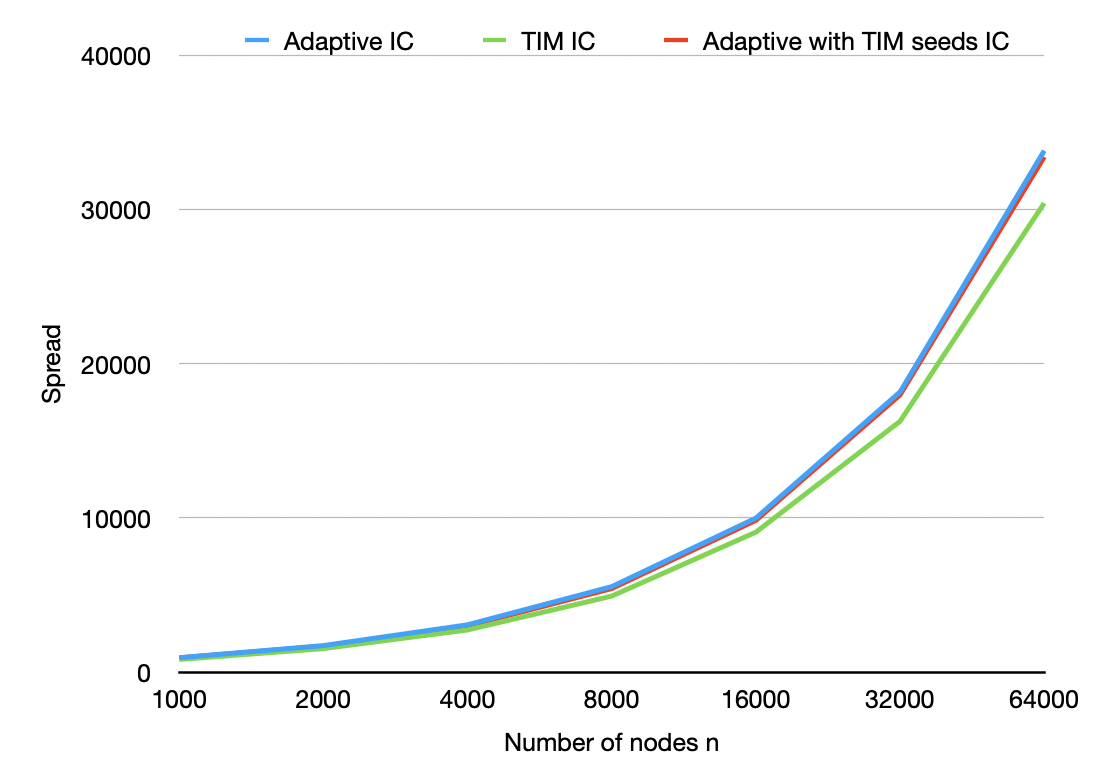
\includegraphics[width=1\linewidth]{GSSI_thesisProposal/figures/ER_IC.png}
    \caption{ER graph; $k=198$}
    \label{fig:first}
\end{subfigure}
\hfill
\begin{subfigure}{0.4\textwidth}
    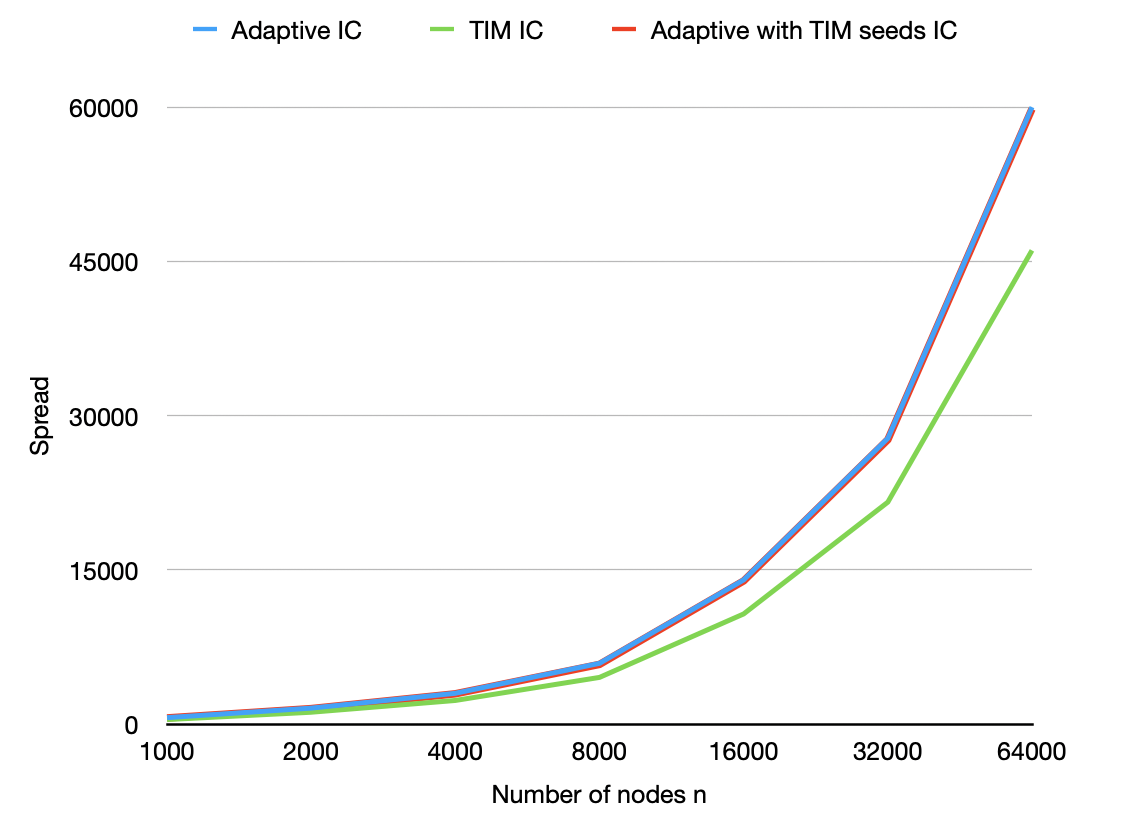
\includegraphics[width=1\linewidth]{GSSI_thesisProposal/figures/WS_IC.png}
    \caption{WS graph; $k=10$}
    \label{fig:second}
\end{subfigure}
\hfill
\begin{subfigure}{0.4\textwidth}
    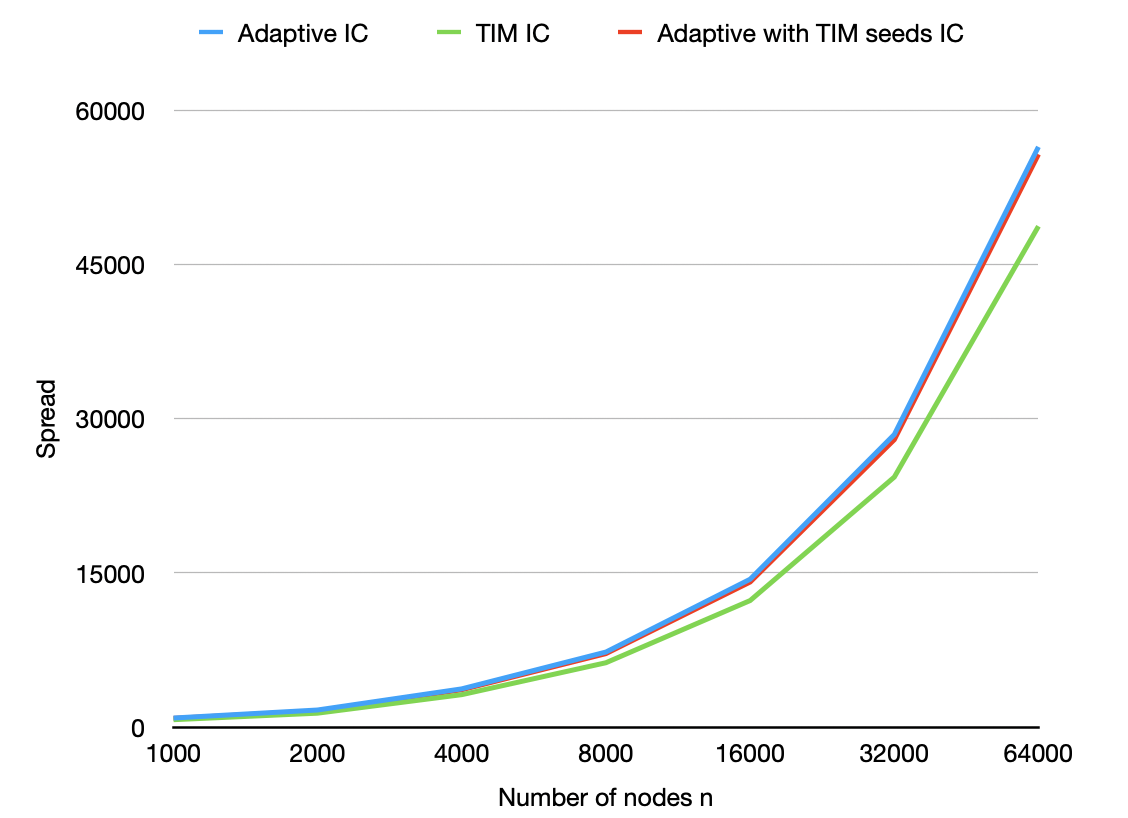
\includegraphics[width=1\linewidth]{GSSI_thesisProposal/figures/BA_IC.png}
    \caption{BA graph; $k=100$}
    \label{fig:third}
\end{subfigure}
\hfill
\begin{subfigure}{0.4\textwidth}
    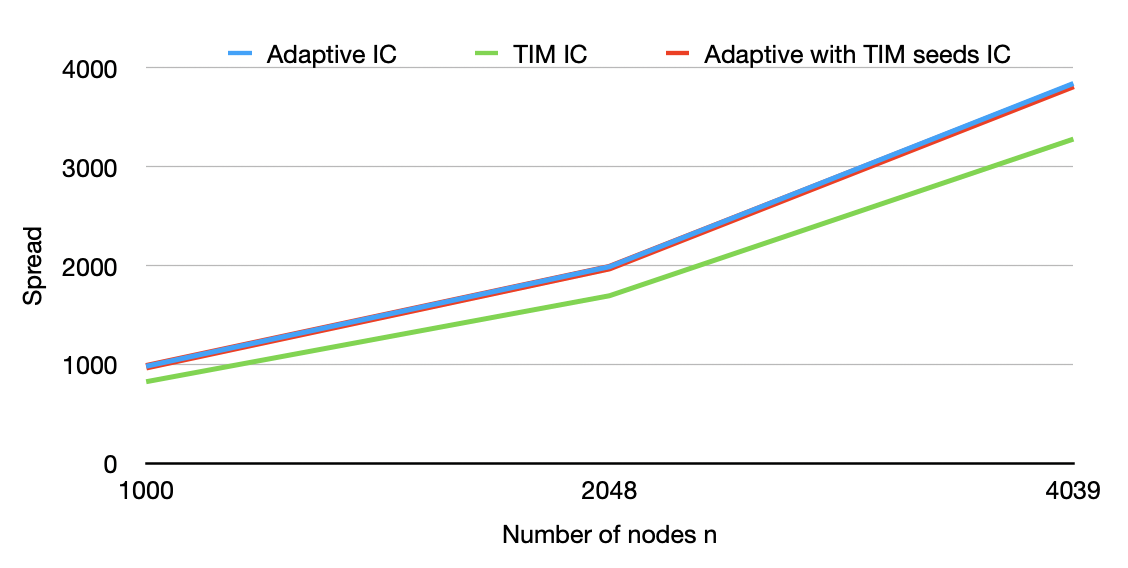
\includegraphics[width=1\linewidth]{GSSI_thesisProposal/figures/Fb_IC.png}
    \caption{Facebook network; $k=50$}
    \label{fig:fourth}
\end{subfigure}
        
\caption{Results under the Independent Cascade model with $p=[0.1,1.0]$.}
\label{fig:figure_IC}
\end{figure}


The figures in \ref{fig:figure_IC} represent the 4 different networks with the edge probability chosen at random between $[0.1,1.0]$. In general, the three generated graphs are comparable to each other with Barabasi-Albert having the best spread. From figure  \ref{fig:figure_IC} and table \ref{AG}, we observe that the seeds selected by the $TIM^+$ algorithm are nearly as good as the ones selected by the adaptive greedy TIM. For comparing the quality of selected seeds that the adaptive greedy TIM and $TIM^+$ produce, we introduce a new algorithm, called the adaptive greedy with TIM seeds, which take the seeds generated by $TIM^+$, but runs them on the same realisations generated by the adaptive greedy TIM. 


 \begin{table} [ht]
    \centering
    \begin{adjustbox}{width=1\textwidth}
    \begin{tabular}{ | c | c | c | c | }
    \hline
    \textit{Graph}& \textit{Greedy Adaptivity Gap}& \textit{Adaptive vs. greedy adaptive (TIM seeds)}& \textit{Greedy adaptive (TIM seeds) vs. $TIM+$}\\[2ex]
     \hline
    Erdős-Rényi& 1.2915& 1.00004& 1.2914\\ [2ex]
    Watts-Strogatz& 1.3024& 1.0031& 1.2983\\[2ex]
    Barabasi-Albert& 1.3155& 1.0068& 1.3067 \\[2ex]
    \hline
    \end{tabular}
    \end{adjustbox}
    \caption{Adaptive ratios with $n=64000$ and $k=10$ under the IC model for generated graphs.}
    \label{AG}
    \end{table}



    \begin{table} [ht]
    \centering
    \begin{adjustbox}{width=1\textwidth}
    \begin{tabular}{ | c | c | c | c | }
    \hline
    \textit{No.of nodes}& \textit{Greedy Adaptivity Gap}& \textit{Adaptive vs. greedy adaptive (TIM seeds)}& \textit{Greedy adaptive (TIM seeds) vs. $TIM+$}\\[2ex]
     \hline
    1000& 1.18872& 1.00497& 1.18285\\ [2ex]
    2048& 1.17294& 1.00458& 1.16759\\[2ex]
    4039& 1.17135& 1.00541& 1.16504\\[2ex]
    \hline
    \end{tabular}
    \end{adjustbox}
    \caption{Adaptive ratios for the Facebook network with $k=50$.}
    \label{FB}
    \end{table}

Table \ref{AG} represents the ratio of the synthetic networks with the three variants of the TIM algorithm, with the greedy adaptivity gap being the ratio between the adaptive greedy TIM and $TIM^+$. Table \ref{FB} shows the three sampled networks of the Facebook graph and their adaptive ratios of the spread, with $k=50$ generated via the TIM algorithms. The ratios are normally higher than $1$ because adaptive algorithms perform strictly better than the non-adaptive ones. The second column is the ratio between the adaptive greedy TIM and the adaptive greedy with the predetermined $TIM^+$ seeds. The ratios in this column tends to 1 which proves that the seeds selected by $TIM^+$ are capable of generating a spread close to its adaptive greedy equivalent. The third column is the column that is similar to the first one, where we compare the greedy adaptive with $TIM^+$ seeds and the $TIM^+$ algorithm. Notice that the values of this column is similar to the greedy adaptivity gap further proving that in this setting, $TIM^+$ seeds are almost as good as the seeds selected by the adaptive greedy policy.




We move on to Figure \ref{fig:figure_int} where we restrain the probability on edges between 0.1 and 0.2 to observe the spread obtained by the three algorithms. From the graph, we see that the seeds selected by $TIM^+$ has a coverage as good as the ones selected by the greedy adaptive policy for both, a synthetic ER graph and a real world Facebook network. We consider these two particular networks to show the difference in activation between a generated graph (ER has a low clustering coefficient which helps to understand the result for low activation probabilities), and the Facebook network represents a real world network. 



\begin{figure}
\centering
\begin{subfigure}{0.4\textwidth}
    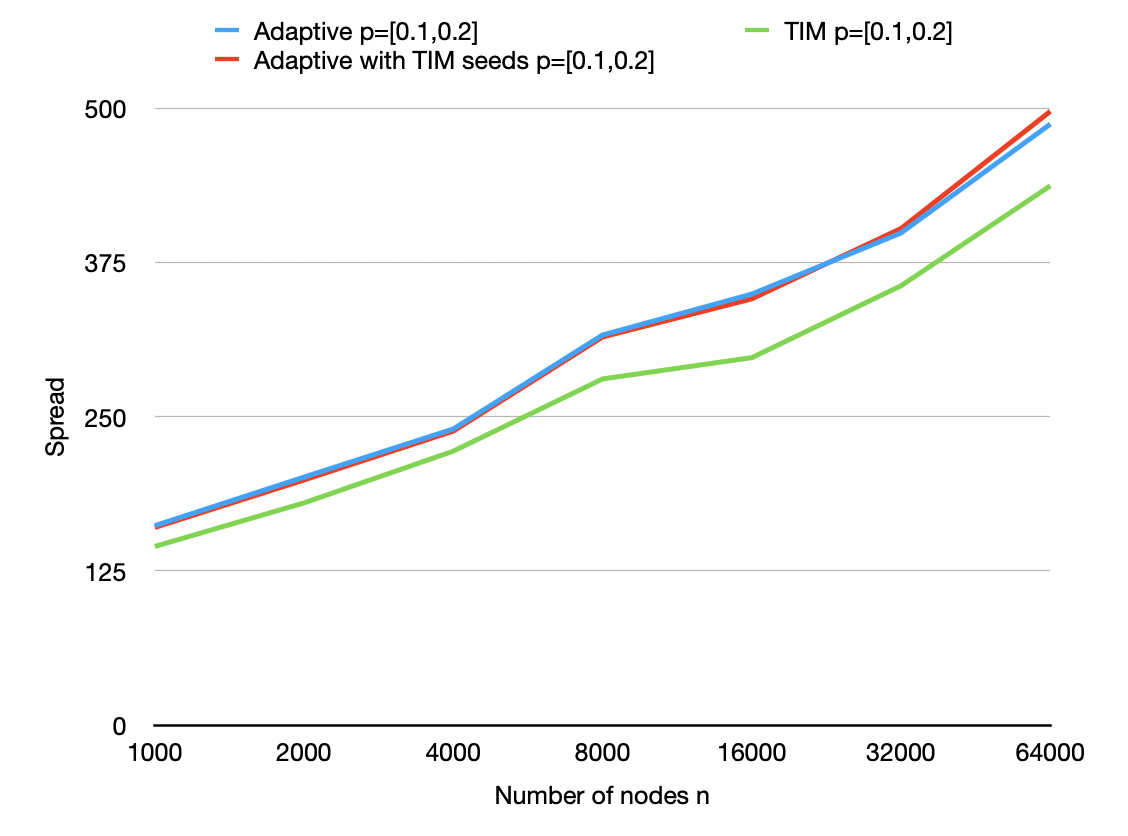
\includegraphics[width=1\linewidth]{GSSI_thesisProposal/figures/ER_int_IC.png}
    \caption{ER graph; $k=49$}
    \label{fig:first_int}
\end{subfigure}
\hfill
\begin{subfigure}{0.4\textwidth}
    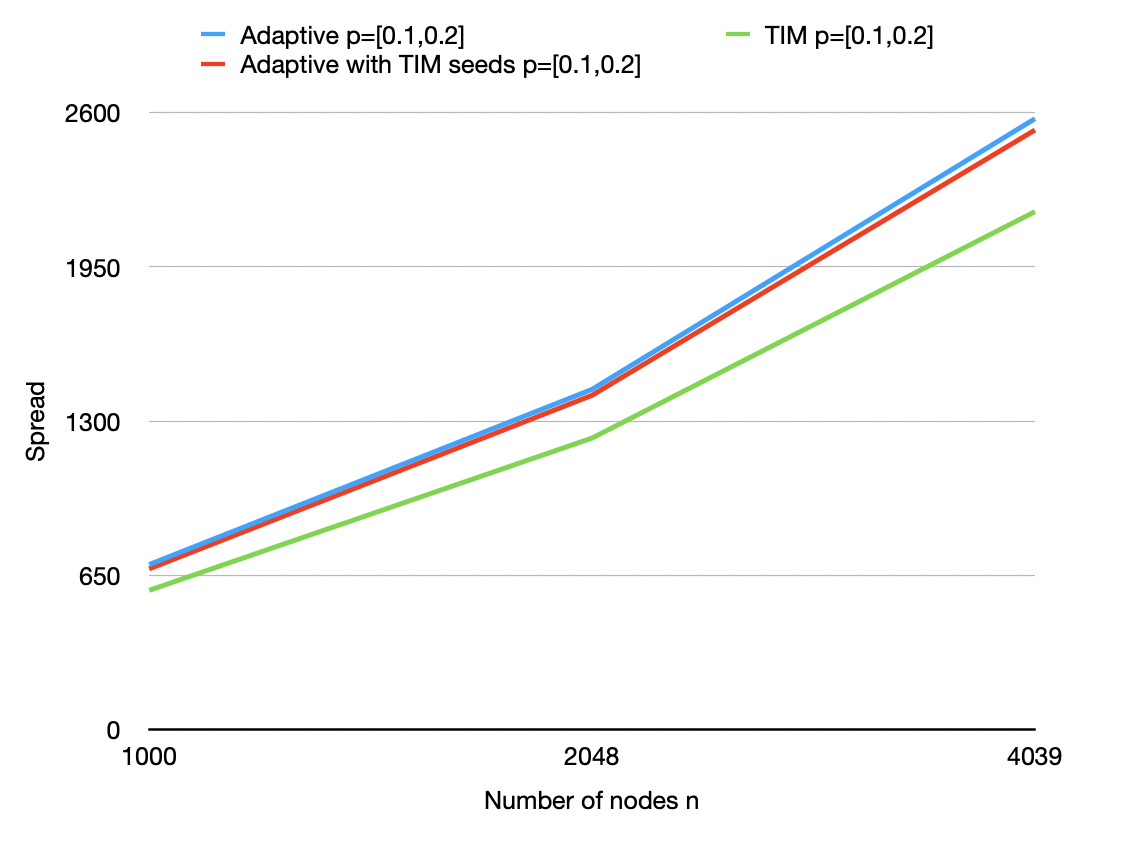
\includegraphics[width=1\linewidth]{GSSI_thesisProposal/figures/Fb_int_IC.png}
    \caption{Facebook network; $k=50$}
    \label{fig:second_int}
\end{subfigure}
\caption{Results under the Independent Cascade model with $p=[0.1,0.2]$.}
\label{fig:figure_int}
\end{figure}


%However, while running the programs, we used two different systems due to the overhead induced by the algorithms. While $TIM^+$ runs faster, the amount of memory required to generate around 200 seeds for a network of size 64000 nodes and 368160 edges (ER graph) is more or less equal to 50GB. Figure \ref{fig:tim_mem} shows the process being killed on a machine with 8GB RAM, when we try to find 30 seeds on a network of size 32000 nodes. Comparing that with figure \ref{fig:aim_mem}, observe that we can run two processes in parallel on a 8GB machine, when we are using the adaptive version of $TIM^+$. In terms of time, the adaptive algorithm with the same parameters took days to run, forcing us to add parallelism to the algorithm since the realisations are independent of each other. We could run three adaptive greedy algorithms in parallel on a machine with 8GB RAM, as shown in figure \ref{fig:aim_mem_er} for an ER graph with 32000 nodes, thus showing us that the adaptive greedy is memory efficient, unlike $TIM^+$.




In the end, since the results generated by the adaptive greedy TIM and $TIM^+$ almost converges, if we want a time efficient seed selection process, we will select $TIM^+$ but at a cost of huge memory overhead. On the other hand, if there is a constraint on the memory, and we need to use a personal computer to run huge networks, an adaptive greedy algorithm is what we want to use, but the time required to run such networks should be calculated in weeks, even when the realisations are run in parallel. 









\subsection{Linear Threshold}

Since the BA graph and the Facebook network have high clustering coefficients, we considered just the same ER and WS graphs we generated for observing the behaviour of LT w.r.t IC. Again, the values of $n$ range from 1000 to 64000. However, the generation of realisations for LT to run the adaptive greedy TIM differs from the IC. 

\paragraph{Parameters.}

The BA graph and most other real world networks are power-law networks, and we observed that the LT model doesn't perform well with these graphs under the adaptive setting. So we consider just ER and WS graphs for the LT. The parameters are the same as in independent cascade with the error parameter $\epsilon = 0.05$. The probability on edges is in between $[0.1,1.0]$ and $k=198$ for ER and $k=10$ for WS, since the WS graph has a high clustering coefficient, which helps in activating almost the entire network with a lesser $k$ value than that of ER. Separate realisations for adaptive TIM are generated according to the underlying LT diffusion model.

\paragraph{Results.}

From figure \ref{fig:second_LT} we immediately notice in the WS graph plot that the $TIM^+$ seeds do not perform as well as it was doing in the IC model. Table \ref{WS} compares the greedy adaptivity gap under both the diffusion models with the same parameters. We observe from the table that the greedy adaptivity gap on average increases by $\approx 65\%$ for the WS network under LT with 10 seeds.


The ER graph plot shows a slight convergence between the red and blue lines representing the spread of adaptive greedy and the adaptive greedy with $TIM^+$ seeds, but the seeds selected by $TIM^+$ still perform quite well when compared to that of WS. To understand why we notice such a deviation can be attributed to the fact that the adaptive greedy TIM is no longer submodular in the LT model, but the theory is not yet proven. The question remains, that experimentally, we see that both models with a high and low clustering coefficient performs better in the LT model as compared to its IC counter part, so is there a way to pass the submodularity requirement in order to reach better theoretical bounds on the adaptivity gap of the linear threshold model with the full-adoption feedback?   


  \begin{table} [ht]
    \centering
    \begin{adjustbox}{width=1\textwidth}
    \begin{tabular}{ | c | c | c | }
    \hline
    \textit{No.of nodes}& \textit{Greedy Adaptivity Gap (IC)}& \textit{Greedy Adaptivity Gap (LT)}\\[2ex]
     \hline
    1000& 1.41086& 2.45217\\ [2ex]
    2000& 1.34130& 3.37854\\[2ex]
    4000& 1.30168& 3.38854\\[2ex]
    8000& 1.30027& 3.51286\\[2ex]
    16000& 1.30840& 4.28206\\[2ex]
    32000& 1.28733& 4.45013\\[2ex]
    64000& 1.30238& 4.32444\\[2ex]
    \hline
    \end{tabular}
    \end{adjustbox}
    \caption{Greedy adaptivity gap for the WS network under IC and LT with $k=10$.}
    \label{WS}
    \end{table}



\begin{figure}
\centering
\begin{subfigure}{0.4\textwidth}
    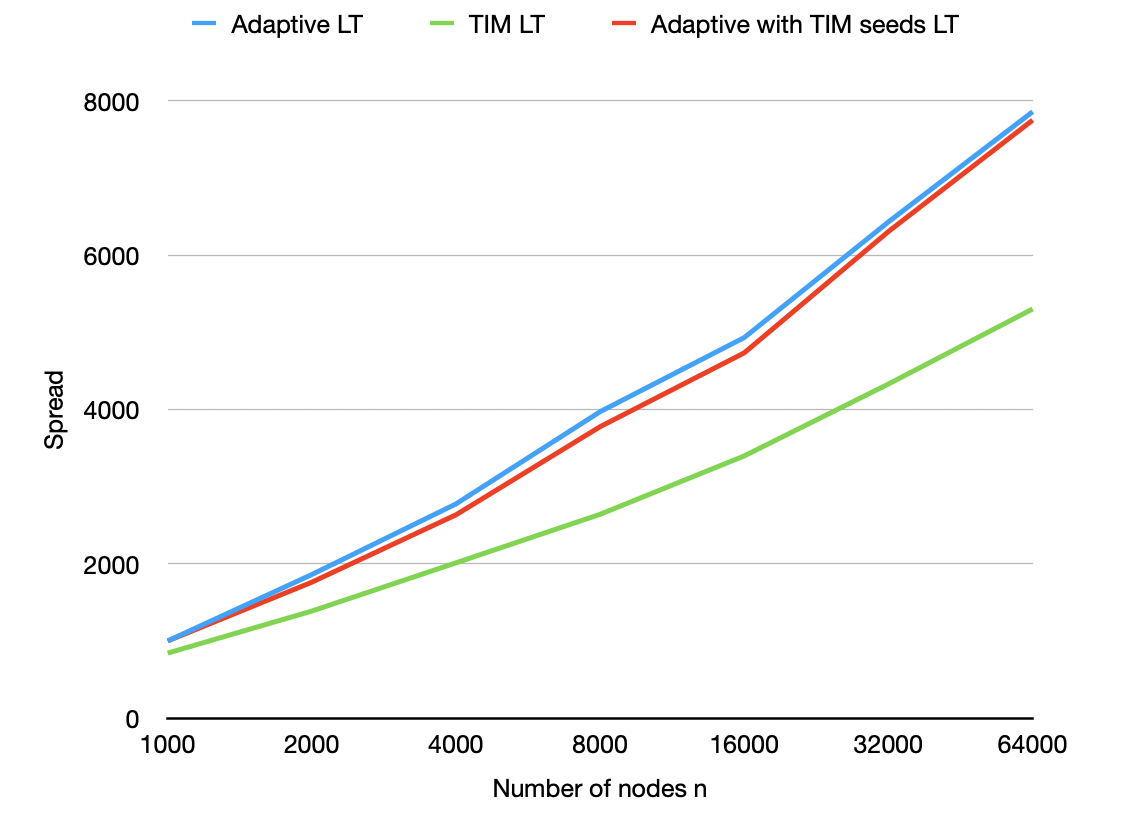
\includegraphics[width=1\linewidth]{GSSI_thesisProposal/figures/ER_LT.png}
    \caption{ER graph; $k=198$}
    \label{fig:first_LT}
\end{subfigure}
\hfill
\begin{subfigure}{0.4\textwidth}
    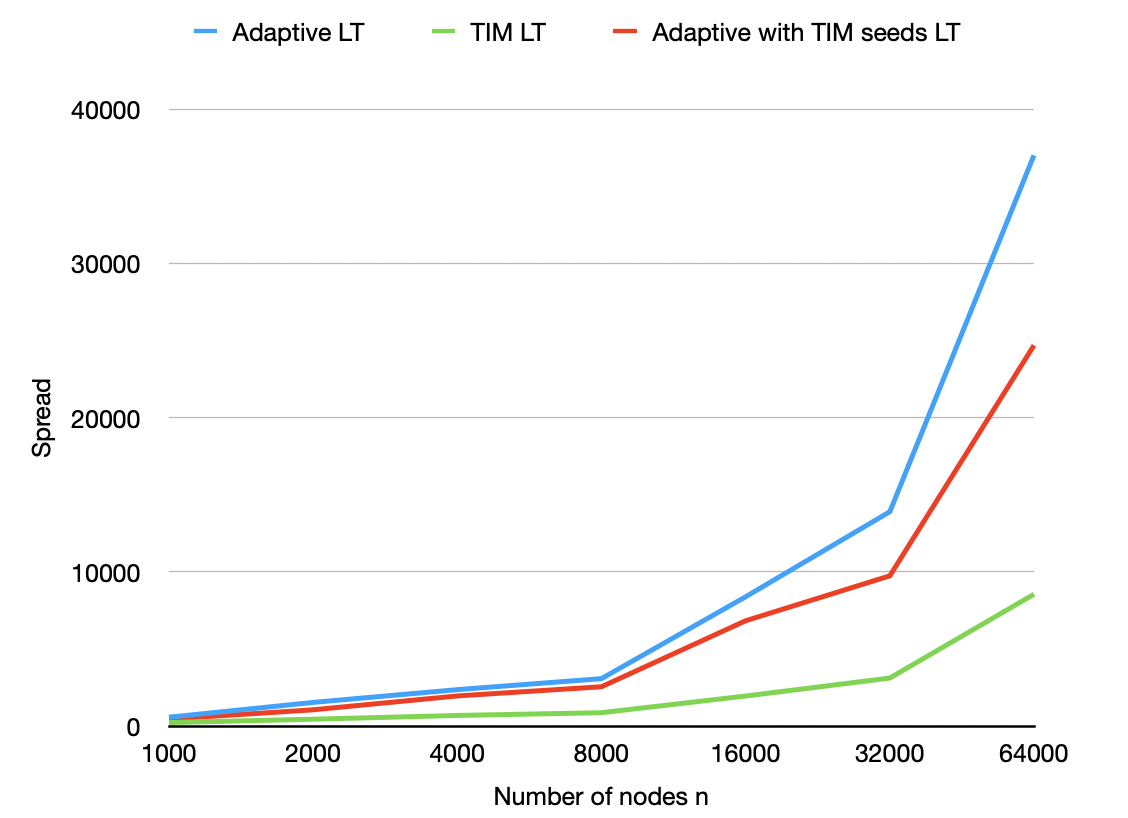
\includegraphics[width=1\linewidth]{GSSI_thesisProposal/figures/WS_LT.png}
    \caption{WS graph; $k=10$}
    \label{fig:second_LT}
\end{subfigure}
\caption{Results under the Linear Threshold model with $p=[0.1,1.0]$.}
\label{fig:figure_LT}
\end{figure}


\section{Summary}\label{sec_future_0}

This chapter studies the adaptivity gap of the independent cascade model with full-adoption feedback. We introduce a new technique to bridge the non-adaptive optimal and the adaptive optimal solution. Our technique directly builds the connection through defining the marginals related to the size $t-1$ non-optimal solution. 

First, we improve on the upper bound of the adaptivity gap for in-arborescences from $2e/(e-1)$ to $2e^2/(e^2-1)$. Second, we give an upper bound of $\lceil n^{1/3} \rceil$ for general graphs, which is the first sub-linear result on general graphs. Third, we show that for a class of $\alpha$-bounded graphs, the adaptivity gap is upper bounded by $\sqrt{\alpha}+O(1)$. Fourth, we prove that for a class of $(\beta,\gamma)$-bounded-activation graphs, we have an adaptivity gap of $\sqrt{\beta}+\frac{1}{1-\gamma}$. All the above results are based on our new technique.

We conduct some experiments on different type of synthetic and real world networks to understand the effect of adaptive greedy with the non-adaptive greedy algorithms. We give an overview of the greedy adaptivity gap to realize that even though the greedy adaptive algorithm is strictly better than the greedy non-adaptive policy, the adaptive greedy policy is not much better than the latter in both the IC and LT diffusion model. The adaptive greedy is memory efficient, whereas the non-adaptive greedy has a better efficiency in time.